\documentclass[prb,twocolumn,superscriptaddress,amsmath,amssymb,longbibliography]{revtex4-2}

\usepackage{graphicx}
\graphicspath{{../figures/}}
\usepackage{siunitx}
\usepackage{booktabs}
\usepackage{xcolor}
\usepackage{hyperref}
\usepackage{multirow}

% Custom commands
\newcommand{\Ecut}{E_{\mathrm{cut}}}
\newcommand{\kpts}{\mathbf{k}}
\newcommand{\xc}{\mathrm{xc}}
\newcommand{\conv}{\mathrm{conv}}
\newcommand{\meth}{\mathrm{method}}
\newcommand{\cert}{\mathcal{C}}
\newcommand{\Nk}{N_k}

\begin{document}

\title{A Posteriori Error Certificates (APECs): \\ Certifying Uncertainty Through the Soft-Mode Bottleneck in  BaTiO$_3$
}

\author{Julien Appleby-Millette}
\email{julienmillette@uvic.ca}
\affiliation{Department of Chemistry, University of Victoria, Victoria, BC, Canada}
\affiliation{Centre for Advanced Materials and Related Technology, University of Victoria, Victoria, BC, Canada}
\author{Kyla Younger}
\affiliation{Department of Chemistry, University of Victoria, Victoria, BC, Canada}
\affiliation{Centre for Advanced Materials and Related Technology, University of Victoria, Victoria, BC, Canada}
\author{Thomas Baker}
\affiliation{Department of Physics \& Astronomy, University of Victoria, Victoria, BC, Canada}
\affiliation{Department of Chemistry, University of Victoria, Victoria, BC, Canada}
\author{Irina Paci}
\email{ipaci@uvic.ca}
\affiliation{Department of Chemistry, University of Victoria, Victoria, BC, Canada}
\affiliation{Centre for Advanced Materials and Related Technology, University of Victoria, Victoria, BC, Canada}

\date{\today}

\begin{abstract}
Density functional theory has become an indispensable tool for predicting functional materials properties, yet computational predictions are rarely accompanied by standardized uncertainty estimates. This limitation is particularly important for derived materials properties, where nonlinear relationships can amplify uncertainties in the underlying electronic structure calculation. Here we introduce A Posteriori Error Certificates (APECs), a method that attaches quantitative uncertainty estimates,  provenance metadata and quality tiers to DFT calculations. Total uncertainty is decomposed into convergence, methodological, intrinsic DFT and model-form contributions. The framework propagates these uncertainties through derived quantities, enabling statistically consistent fusion of heterogeneous computational data. We demonstrate the approach for a challenging problem, the electro-optic response of 
tetragonal BaTiO$_3$, where the inverse-square dependence of the Pockels coefficient on the soft-mode frequency amplifies modest uncertainties in phonon calculations. Twelve certificates are extracted from a production DFPT 
calculation and combined  with cross-functional literature data. Phase-aware 
partitioning  resolves inconsistencies arising from mixed crystallographic phases and tensor conventions, yielding a fused electro-optic coefficient within 3\% of the bulk experimental value, while reducing the uncertainty from 27\% for a single calculation to 20\% through principled data fusion. Broadly, APECs provide a methodology for uncertainty-aware computational materials design, enabling calculated properties to be compared, combined, propagated through multiscale workflows, and reused reliably. 
\end{abstract}

\maketitle

%%%%%%%%%%%%%%%%%%%%%%%%%%%%%%%%%%%%%%%%%%%%%%%%%%%%%%%%%%%%%%%%%%%%%%%%%%%%%%%
\section{Introduction}
\label{sec:intro}
%%%%%%%%%%%%%%%%%%%%%%%%%%%%%%%%%%%%%%%%%%%%%%%%%%%%%%%%%%%%%%%%%%%%%%%%%%%%%%%

Barium titanate (BaTiO$_3$) is among the most promising materials for 
integrated electro-optical modulators, offering Pockels coefficients an order of 
magnitude greater than lithium niobate and compatibility with silicon photonic 
platforms \cite{Abel2019,Eltes2020,Lines2001}. Predicting the 
electro-optic response from DFT is therefore a problem of direct 
technological significance. It is also a problem that exposes a fundamental 
weakness in how computational materials science handles uncertainty: standard methodological errors in DFT are often amplified when calculating derived properties.

The Pockels coefficient $r_{33}$ of BaTiO$_3$ depends on the soft transverse 
optical phonon frequency $\omega_{\mathrm{soft}}$ through an inverse-square 
relationship \cite{Veithen2005}, 
\begin{equation}
    r_{33} \propto \frac{Z^{*2}}{\omega_{\mathrm{soft}}^2}
    \label{eq:soft_mode}
\end{equation}
 where $Z^*$ is the Born effective charge. A modest 5\% 
 uncertainty in $\omega_{\mathrm{soft}}$, well within the variation among standard 
exchange-correlation functionals, becomes a 10\% uncertainty in $r_{33}$. 
The published DFT values of $r_{33}$ for bulk  BaTiO$_3$ vary by a factor of two or more 
depending on the functional \cite{Veithen2005,Wahl2008,Bilc2008}, 
reflecting the increased sensitivity to $\omega_{\mathrm{soft}}$. Near the 
Curie temperature, where $\omega_{\mathrm{soft}} \to 0$, this amplification 
diverges entirely.

This amplification is not unique to BaTiO$_3$ Pockels coefficients or ferroelectrics. Any property 
with nonlinear dependence on DFT outputs will behave similarly: piezoelectric coefficients depend on phonon frequencies and Born 
charges \cite{Wu2005_piezo}, defect formation energies enter 
Arrhenius rates exponentially \cite{Freysoldt2014}, and catalytic 
turnover frequencies depend exponentially on adsorption energies 
\cite{Norskov2004,Medford2015}. In each case, modest input uncertainties 
propagate into large output uncertainties through the physics of the problem. Our group encountered similar challenges in electronic structure calculations of response properties in heterogeneous nanocomposites, where subtle changes in electronic structure, inclusion morphology, and interfacial polarization can produce significant changes in the predicted material response \cite{Rowan2011,Henderson2023}.

Yet, no standardized quantification of uncertainty in DFT calculations exists \cite{Burke2012}. Predicted properties often vary widely with the choice of exchange-correlation functionals, basis sets and convergence parameters. Of particular relevance for materials calculations are band gaps. These are often underestimated by LDA and GGA functionals by 
35 -- 40\%, whereas hybrid functionals vary by $\pm$15\% 
depending on the proportion of exact exchange included \cite{Borlido2019,Heyd2003_HSE}.  Even lattice constants differ systematically across functionals with variations of the order of 0.5\% 
\cite{Lejaeghere2016,Haas2009}, whereas formation energies for transition metal oxides show spreads of 0.1 -- 0.3 eV\cite{Kingsbury2022,Stevanovic2012_FERE}, and elastic constants show variations of 10 -- 30\%  for complex materials 
\cite{deJong2015}.

This heterogeneity becomes a systemic problem as computational materials 
science scales. Large computational materials databases (Materials Project, AFLOW, JARVIS) aggregate millions of entries generated using different computational approximations \cite{Jain2013, Curtarolo2012,Choudhary2020,Kirklin2015_OQMD,Draxl2019_NOMAD,Andersen2021_OPTIMADE}. These results are often treated on equal footing in data-driven approaches such as machine learning, despite potentially significant differences in reliability and systematic errors or biases \cite{Bartel2020_critical_ML}.    
%now contains over 150,000 inorganic compounds \cite{Jain2013}, AFLOW exceeds 3.5 million entries \cite{Curtarolo2012}, and JARVIS provides multi-fidelity data across DFT, classical, and machine learning methods \cite{Choudhary2020,Saal2013_OQMD,Kirklin2015_OQMD,Draxl2019_NOMAD,Andersen2021_OPTIMADE}. When machine learning models train on databases aggregating such heterogeneous calculations, they inherit these inconsistencies as noise, leading to degraded accuracy and miscalibrated uncertainty estimates\cite{Faber2016,Xie2018_CGCNN,Chen2019_CGCNN,Bartel2020_critical_ML}. A researcher who downloads 100,000 compounds from a materials database, trains a graph neural network, and reports a test MAE of 30~meV/atom has no way to separate model error from label noise---some entries are well-converged ($\sigma \sim 5$~meV/atom) while others are screening-quality ($\sigma \sim 50$~meV/atom), and functional biases differ systematically by chemistry.

Several prior approaches have been devised to address DFT uncertainty. The $\Delta$-project \cite{Lejaeghere2016} and subsequent automated convergence 
workflows \cite{Bosoni2024_ACWF} established that different DFT codes agree to 
within $\sim$ 1~meV/atom when using identical parameters, demonstrating that 
\emph{implementation} differences are negligible and that the dominant 
uncertainty source is the choice of method, not the choice of code. 
The BEEF-vdW functional ensemble \cite{Wellendorff2012,Pandey2015_mBEEF} 
estimates methodological uncertainty directly through Bayesian sampling of 
exchange-correlation functionals, but is restricted to the BEEF family 
and cannot be applied retrospectively to existing datasets. %(though where available, BEEF-derived $\sigma_\meth$ estimates can be incorporated into the certificate schema). 
Statistical models by Pernot et al. 
 \cite{Pernot2015,Pernot2020,Simm2016} calculate intrinsic and systematic errors across properties and functionals, providing an empirical basis for uncertainty estimates, but not 
a per-calculation representation. 
At the database level, ad hoc correction schemes such as the GGA/GGA+$U$ 
mixing for transition metal 
oxides \cite{Jain2011_GGA_U,Wang2006_oxidation,Hautier2012} improve accuracy but do not provide uncertainty estimates for individual entries. Finally, automated convergence 
frameworks \cite{Huber2020_AiiDA,Wisesa2016,Mathew2017_atomate,Ong2013_pymatgen} 
educe the cost of numerical validation but yield pass/fail criteria rather than quantitative uncertainty measures.

Here, we introduce a methodology that treats uncertainty as structured metadata attached to computational materials data. Rather than being tied to a particular exchange-correlation functional, workflow or dataset, the resulting A Posteriori Error Certificates (APECs) can be generated retrospectively for completed calculations and incorporated into existing databases. Each computed quantity of interest is provided with an uncertainty certificate. The certificate decomposes uncertainty into convergence, methodological, intrinsic DFT and model-form contributions, records computational provenance, and assigns a quality tier. The approach also provides a means of propagating these uncertainties through derived quantities and combining results across heterogeneous sources in a consistent manner. 
%that attaches quantitative error estimates as metadata to DFT-generated data and compounded properties. Each computed quantity is associated with an uncertainty estimate, decomposed into contributions such as convergence, methodological choices and intrinsic DFT limitations. The uncertainties are reported together with the computed values or can be added to existing data, and are then classified into discrete quality tiers, enabling comparisons between distinct calculations. Moreover, the approach (discussed in the following pages as the Posterior Error Certificates approach) provides a  means to propagate uncertainties through derived quantities and combine results from diverse sources in a consistent manner.    %\emph{posterior error certificates}---standardized metadata structures that attach decomposed uncertainty estimates to DFT-computed  properties. The framework decomposes uncertainty into convergence error ($\sigma_\conv$), methodological spread ($\sigma_\meth$), intrinsic DFT limitations ($\sigma_{\mathrm{DFT}}$), and---for derived properties that depend on phenomenological models---model-form error ($\sigma_{\mathrm{model}}$). It assigns discrete quality tiers (red/amber/green) that enable filtering and trust calibration across heterogeneous datasets, and provides a propagation calculus that tracks uncertainty through derived quantities and multi-stage computational workflows. Cross-method normalization is achieved through inverse-variance weighting, bias correction, and hierarchical Bayesian modeling.

We apply the methodology to the electro-optic response of BaTiO$_3$, a system in which the soft-mode amplification of errors, propagated into the evaluation of the electro-optic tensor, makes  uncertainty 
quantification essential. Using a reference DFPT calculation, we extract twelve 
 certificates spanning structural, charge-response, dielectric, 
phonon, and derived electro-optic properties. 
%(the latter in both $zz$ and isotropic tensor conventions). 
We demonstrate phase-aware fusion of heterogeneous data sources and quantify the resulting reduction in uncertainty. 
We assign to these values an expected quality tier: green for well-converged ground-state properties, amber for 
response properties, and red for the derived Pockels coefficient subject 
to both propagated uncertainty and model-form error. The BaTiO$_3$ case study serves both as a validation of the certificate framework and as an illustration of how uncertainty-aware data aggregation can enhance the reliability of computational predictions of materials properties. 


%%%%%%%%%%%%%%%%%%%%%%%%%%%%%%%%%%%%%%%%%%%%%%%%%%%%%%%%%%%%%%%%%%%%%%%%%%%%%%%
%\section{Case Study: Electro-Optic Tensors in BaTiO$_3$}
\section{Results}
\label{sec:results}
%%%%%%%%%%%%%%%%%%%%%%%%%%%%%%%%%%%%%%%%%%%%%%%%%%%%%%%%%%%%%%%%%%%%%%%%%%%%%%%

%We demonstrate the certificate framework on a challenging application: the  Pockels tensor in barium titanate (BaTiO$_3$), where nonlinear physics amplifies DFT uncertainty and makes rigorous uncertainty quantification essential.

%\subsection{Soft Mode Amplification in BaTiO$_3$}

The APECs method assigns uncertainty certificates to individual DFT-calculated and derived quantities, and enables their combination across heterogeneous data sources. We demonstrate the workflow using a challenging application: the Pockels tensor in BaTiO$_3$. We build the certificates from calculated, literature and database data, quantifying the dominant uncertainty contributions. Specifically, in the following pages we generate certificates for a production DFPT calculation and examine how library fusion and provenance-aware partitioning affect the resulting electro-optic effect. 

In BaTiO$_3$, a transverse optical phonon mode softens as temperature approaches the Curie point $T_C \approx 400$~K \cite{Lines2001,Cochran1960,Zhong1994_BTO,Zhong1995}. The change in the refractive index of the material with an applied electric field is determined by the Pockels coefficient $r_{33}$ which depends on this soft-mode frequency as discussed in Equation \ref{eq:soft_mode}. More specifically \cite{Veithen2005},
%To calculate the electro-optic coefficient $r_{33}$ we use the calibrated soft-mode expression \cite{Veithen2005}
\begin{equation}
    r_{33} = r_{\mathrm{ref}} \times \left(\frac{\omega_{\mathrm{ref}}}{\omega }\right)^2\times 
\left(\frac{Z^*}{Z^*_{\mathrm{ref}}}\right)^2 \times 
\left(\frac{\varepsilon_{\mathrm{ref}}}{\varepsilon^\infty}\right).
\label{eq:soft_mode_reference}
\end{equation}
Here, $Z^*$ is the Born effective charge associated with the soft polar mode
\cite{Ghosez1998_BEC,Resta1994_BEC,KingSmith1993}. Reference values are the 
bulk experimental value of Zgonik et al.\ \cite{Zgonik1994}
$r_{\mathrm{ref}} = 105$~pm/V, $\omega_{\mathrm{ref}} = 180$~cm$^{-1}$ 
\cite{Lines2001}, $Z^*_{\mathrm{ref}} = 7.16$~$e$ 
\cite{Ghosez1998_BEC}, and $\varepsilon_{\mathrm{ref}} = 6.5$ 
\cite{Ghosez1998_BEC}. 

Uncertainty in the quantities entering Equation~\ref{eq:soft_mode_reference}
propagates into the derived electro-optic response according to:
\begin{equation}
\left(\frac{\sigma_{r_{33}}}{r_{33}}\right)^2
=
\left(2\frac{\sigma_{\omega}}{\omega_{\mathrm{soft}}}\right)^2
+
\left(2\frac{\sigma_{Z^*}}{Z^*}\right)^2
+
\left(\frac{\sigma_{\varepsilon}}{\varepsilon_{\infty}}\right)^2 .
\label{eq:r33_uncertainty}
\end{equation}

%Within the APECs framework, the uncertainty associated with each input quantity is further decomposed into convergence ($\sigma_{\mathrm{conv}}$), methodological($\sigma_{\mathrm{method}}$), intrinsic DFT($\sigma_{\mathrm{DFT}}$), and model-form ($\sigma_{\mathrm{model}}$) contributions.

%This inverse-square relationship creates uncertainty amplification:
%\begin{equation}
%    \frac{\delta r_{33}}{r_{33}} = 2 \frac{\delta\omega}{\omega_{\mathrm{soft}}}
%    \label{eq:amplification}
%\end{equation}

%A modest 5\% uncertainty in $\omega_{\mathrm{soft}}$ thus becomes 10\% uncertainty in $r_{33}$. Near $T_C$, where $\omega_{\mathrm{soft}} \to 0$, this amplification diverges---making BaTiO$_3$ an ideal stress test for any uncertainty quantification framework.

Each quantity appearing in Equation~\ref{eq:soft_mode_reference} is associated with an APEC, a structured metadata record that attaches quantitative uncertainty estimates to DFT-computed and derived properties. The method decomposes uncertainty for each property (such as the ones in Equation \ref{eq:r33_uncertainty}) into convergence uncertainty ($\sigma_{\mathrm{conv}}$), methodological uncertainty ($\sigma_{\mathrm{method}}$), intrinsic DFT uncertainty ($\sigma_{\mathrm{DFT}}$), and, for derived quantities, model-form uncertainty ($\sigma_{\mathrm{model}}$):
\begin{equation}
\sigma_{\rm total}
=
\sqrt{
\sigma_{\rm conv}^2+
\sigma_{\rm method}^2+
\sigma_{\rm DFT}^2+
\sigma_{\rm model}^2
}, 
\label{eq:sigma_sum}
\end{equation}
\noindent where $\sigma_{\rm total}$ denotes the total uncertainty
associated with a given observable, such as
$\sigma_{r_{33}}$, $\sigma_{\omega}$,
$\sigma_{Z^*}$, or $\sigma_{\varepsilon}$. 

These uncertainties are reported together with the computed values and provenance metadata, can be added to existing data, and are classified into discrete quality tiers (Red/Amber/Green) that facilitate comparison across calculations and data sources. The certificates further provide a mechanism for propagating uncertainty through derived quantities and for combining information from heterogeneous literature and database sources in a consistent manner.

\subsection{Extracting Certificates from Literature and Database Sources}

To construct APECs for BaTiO$_3$, literature values and computational data were collected from published studies and public materials databases.
 We developed workflows for data extraction and retroactive uncertainty estimation for three 
source types: a literature compilation from published 
DFPT studies spanning 1994--2025 \cite{Baroni2001,Gonze1997_DFPT}, Materials Project entries 
(mp-5986 for the tetragonal phase, mp-2998 for cubic) with automated 
uncertainty estimation, and the Kyoto PhononDB with systematic phonon 
calculations \cite{Togo2015_phonopy,Togo2023_PhononDB}.
Most DFT data in these public repositories is reported without uncertainty 
estimation. The present workflow constructs APECs from the reported computational settings, convergence behaviour and cross-functional comparisons where available. 

%\paragraph{Handling Incomplete Data.}

Public databases also typically lack explicit convergence uncertainty information. Our method applies a hierarchy of increasingly conservative estimation strategies to address this. When cutoff and $k$-point parameters are reported but convergence tests are unavailable, we assign representative convergence estimates (see Supplemental Material Tables~S3--S4) using typical convergence behavior in perovskite DFPT calculations, informed by published convergence studies ~\cite{Ghosez1999,Wahl2008} and cross-checked against our own BaTiO$_3$ calculations. 
These estimated ranges are provisional rather than universal, and should be refined as systematic convergence benchmarks become available. 
When calculations of the same property are available for multiple functionals, the cross-functional spread provides a direct estimate of $\sigma_\meth$ via Equation \ref{eq:method_spread}. Missing metadata automatically triggers quality tier downgrading from Green to Amber or Red.
%, with appropriate flags for downstream users. 
All values carry provenance metadata, indicating whether the uncertainty is derived from a convergence test, a literature range, or a heuristic estimate.

%\paragraph{BaTiO$_3$ Literature Library.}

The compiled literature library serves as an empirical reference distribution against which  
new BaTiO$_3$ calculations can be compared and cross-validated. 
By aggregating values from 
multiple groups, codes, and functionals over three decades of DFPT work, the data 
capture the empirical spread that defines methodological uncertainty and 
provides the multi-source inputs needed for inverse-variance weighted 
averaging. Table~\ref{tab:literature_library} summarizes  these data, including recent 
cross-functional comparisons \cite{Amounas2024,Inerbaev2025} and our own 
production calculations. The library includes entries 
spanning three  
exchange-correlation functionals (LDA, PBE, PBEsol),
and experimental 
references, along with experimental Pockels coefficient measurements from 
bulk crystals and epitaxial thin 
films \cite{Reynaud2025,Suceava2025,Ghosez1998_BEC,Zhong1994_BTO,Veithen2005,Kwei1993,Hewat1973}. In particular, the  $Z^*_{\mathrm{Ti}}$ and $\varepsilon^\infty$ entries illustrate the 
importance of phase-aware partitioning: cubic-phase values differ significantly 
from tetragonal-phase values for the same descriptor.

\begin{table*}
\centering
\caption{BaTiO$_3$ library summary. Best estimate values are weighted averages within each reported subset. 
}
\label{tab:literature_library}
\begin{tabular}{llccl}
\toprule
Parameter & Phase & Sources & Functionals & Best estimate \\
\midrule
$Z^*_{\mathrm{Ti}}$ (isotropic) & Cubic & 4 DFT & LDA, PBE & $7.27 \pm 0.17$ \\
$Z^*_{\mathrm{Ti},zz}$ & Tetragonal & 1 DFT & PBE & $6.20 \pm 0.20$ \\
$\varepsilon^\infty$ (avg) & Tetragonal & 3 DFT & LDA, PBE & $6.77 \pm 0.14$ \\
$\varepsilon^\infty_{zz}$ & Tetragonal & 1 DFT & PBE & $5.96 \pm 0.18$ \\
$\omega_{\mathrm{soft}}$ & Tetragonal & 5 DFT & ~ LDA, PBE, PBEsol~ & $176 \pm 6$ cm$^{-1}$ \\
$P_s$ & Tetragonal & ~ 3 DFT, 1 Expt ~ & ~ LDA, PBE, PBEsol ~& $0.27 \pm 0.02$ C/m$^2$ \\
$c/a$ & Tetragonal & ~ 3 DFT, 1 Expt ~ & ~ LDA, PBE, PBEsol ~& $1.011 \pm 0.003$ \\
$a$ (lattice) & Tetragonal & ~ 4 DFT, 1 Expt ~ & ~ LDA, PBE, PBEsol ~ & $3.993 \pm 0.015$ \AA \\
\bottomrule
\end{tabular}
\end{table*}

%This library enables weighted averaging across heterogeneous sources and functional-specific bias estimation. New calculations can be cross-validated against established values, and temporal trends in methodology can be tracked as the compilation grows.

\subsection{Convergence Analysis}

Different uncertainty sources dominate different observables in BaTiO$_3$. Structural quantities converge relatively rapidly with respect to cutoff energy and k-point sampling, whereas response properties remain substantially more sensitive to numerical and methodological choices \cite{Hally2018}. Convergence analysis helps identify which computational parameters limit the accuracy for each quantity entering the calculation of the Pockels coefficient, and where additional computational investment will or will not reduce uncertainty. 

{\bf Soft-Mode Frequency.}
The soft-mode frequency is the most convergence-sensitive input to the 
Pockels coefficient, requiring significantly higher cutoff energies and 
denser $k$-point meshes than structural properties. 
Figure~\ref{fig:omega_convergence} shows the estimated convergence behaviour of $\omega_{\mathrm{soft}}$ 
based on the parametric models described by Equations ~\ref{eq:cutoff_model} 
and~\ref{eq:kpoint_model}. The soft-mode frequency 
converges more slowly than total energy or forces, requiring $\Ecut > 80$~Ry 
for $<2\%$ error and a $k$-point mesh of $8\times8\times8$ or denser. At 
the parameters used in our production calculation (60~Ry, $6\times6\times6$), the 
estimated convergence uncertainty is $\sigma_\omega/\omega \approx 3\%$, 
consistent with the heuristic estimates in 
Supplemental Material Table~S4.

\begin{figure*}
\centering
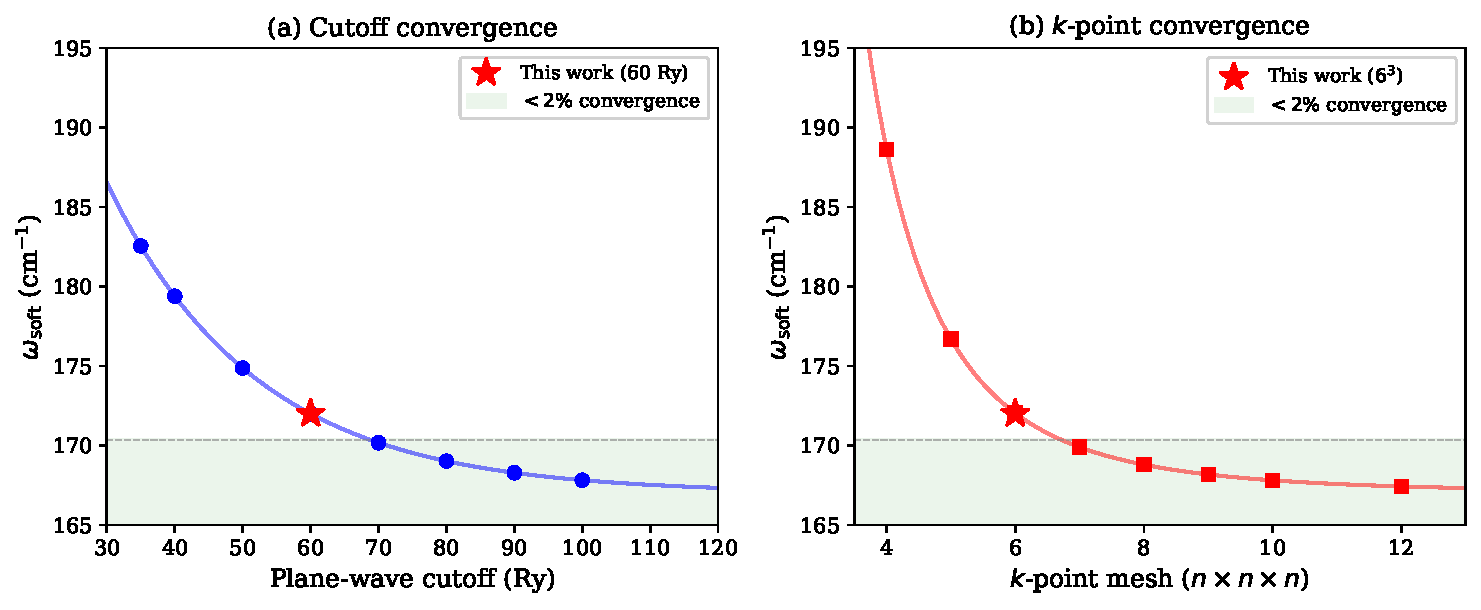
\includegraphics[width=\textwidth]{fig1_omega_convergence.pdf}
\caption{Model-based convergence estimates for the soft-mode frequency in 
BaTiO$_3$. Equations ~\ref{eq:cutoff_model} 
and~\ref{eq:kpoint_model} are used, with preliminary parameters for the perovskite 
oxide class shown in Supplemental Material Table~S3. Curves are estimates from the fitted models, not explicit convergence calculations at every point. Stars mark the  
evaluation at the production calculation parameters (PBE/PAW, 60~Ry, $6^3$ 
$k$-points). The green band indicates the $<2\%$ convergence region. }
\label{fig:omega_convergence}
\end{figure*}

{\bf Born Effective Charges.}
Born effective charges converge more rapidly than the soft mode. At 60 Ry,  
$\sigma_{Z^*}/Z^* < 1\%$ is already achieved, with relatively weak dependence on k-point sampling. Unlike the soft-mode frequency, the Born charges therefore contribute only modestly to the convergence component of the final r$_{33}$ certificate.

{\bf Propagated Uncertainty in $r_{33}$.}
The key question
is how convergence uncertainties in the individual in-
puts propagate into the derived Pockels coefficient.
Applying Equation~\ref{eq:r33_uncertainty} with
$\sigma_\omega/\omega \approx 3\%$ and
$\sigma_{Z^*}/Z^* \approx 1\%$ yields a propagated
uncertainty of approximately 6.3\%.

The soft-mode convergence dominates the propagated
uncertainty, as expected from the sensitivity analysis.
Including $\varepsilon_\infty$ convergence from
Equation~\ref{eq:r33_uncertainty} (1.5\%, entering
with exponent 1) gives
$\sigma_{\mathrm{conv}} = 6.5\%$ for $r_{33}$.



\subsection{Independent SCF Convergence Study}

To validate the convergence estimates  against explicit calculations, we
performed an independent Quantum ESPRESSO SCF convergence study for the
same 40-atom tetragonal BaTiO$_3$ supercell used in the certificate workflow, shown in Figure \ref{fig:scf_convergence}.
The study includes 37 single-point calculations using the PBE and PBEsol functionals, with systematic variation of both plane-wave cutoff and Monkhorst-Pack k-point sampling. 
%from 30--90~Ry over $4^3$, $6^3$, $8^3$, and $10^3$ Monkhorst--Pack meshes, and PBEsol from 40--80~Ry over $4^3$, $6^3$, and $8^3$ meshes. 
All runs converged to
SCF residuals below $10^{-10}$~Ry, and the highest-cutoff/highest-$k$ case within
each functional is used as the internal reference for the corresponding
functional. 

\begin{figure*}
\centering
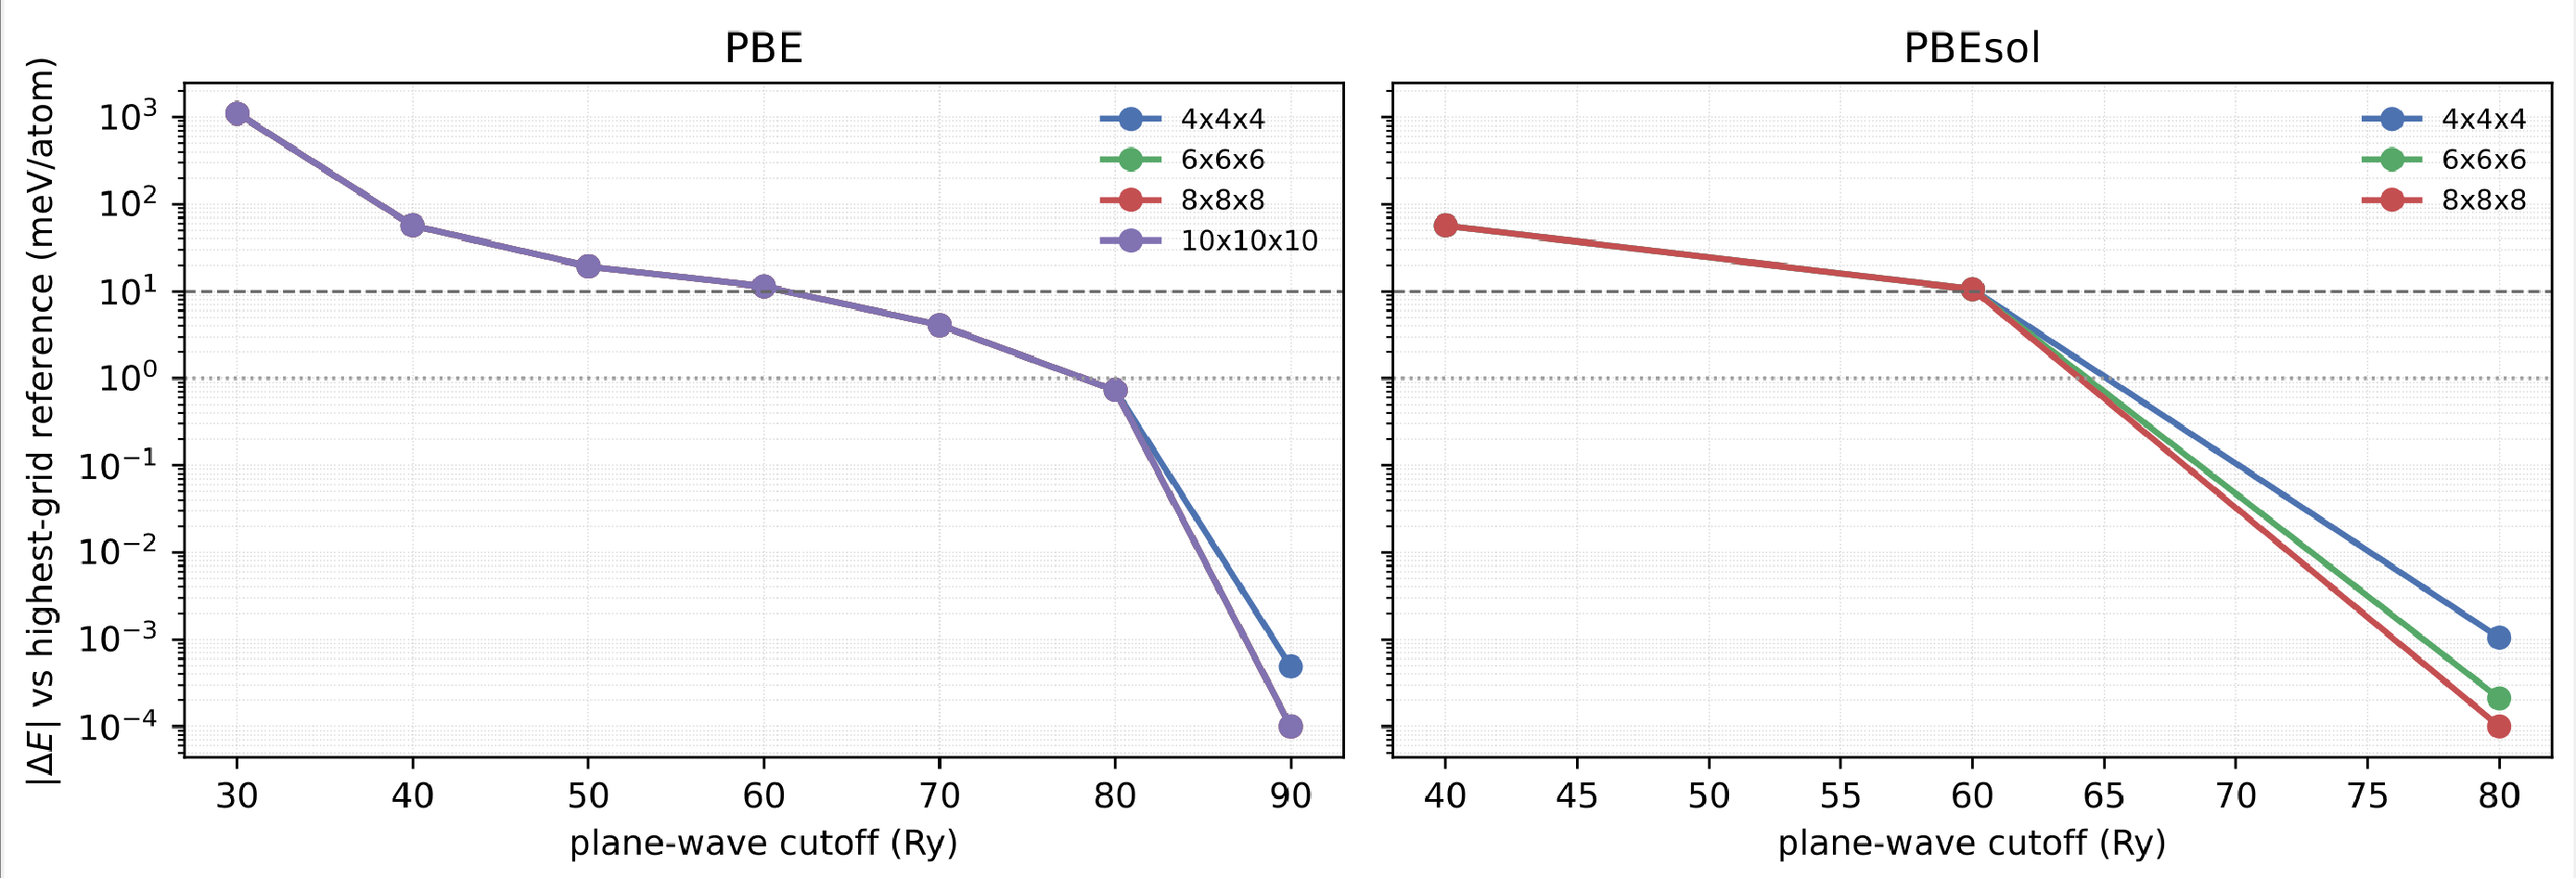
\includegraphics[width=\textwidth]{fig4_scf_convergence.pdf}
\caption{SCF total-energy convergence study for the 40-atom
tetragonal BaTiO$_3$ supercell. 
Energies are shown relative to the highest-cutoff, densest-$k$-point calculations performed for each functional (PBE: 90~Ry, $10
\times 10\times 10$; PBEsol: 80~Ry, $8\times 8 \times 8$). 
The dashed and dotted
horizontal lines mark 10 and 1~meV/atom thresholds. Energy convergence is dominated by the plane-wave cutoff, whereas the residual k-point dependence at the highest cutoff is
below $2\times10^{-3}$~meV/atom.}
\label{fig:scf_convergence}
\end{figure*}

The convergence study shows that the total energy for this supercell controlled primarily by the plane-wave cutoff rather than
by k-point sampling. For both PBE and PBEsol, the production-like 60~Ry, $6\times6\times 6$ 
calculations remain approximately 10 -- 11 ~meV/atom above the highest-cutoff reference calculations, while increasing the cutoff to 80~Ry reduces the residual error below 1~meV/atom across all sampled k-point meshes. 
%For PBEsol, the corresponding 60~Ry, $6\times\6\times 6$ point lies 10.5 ~meV/atom above the 80~Ry, $8\times8\times8$ reference, and80~Ry again brings the sampled grid below 1~meV/atom. 
By contrast, the residual variation
among k-point meshes at the maximum cutoff is negligible (roughly 10$^{-3}$ meV/atom for both PBE and PBEsol).
%$5.7\times10^{-4}$~meV/atom for PBE and $1.3\times10^{-3}$~meV/atom for PBEsol. 
These results support the use of conservative cutoff-driven convergence
uncertainties for structural and total-energy quantities, while also illustrating
why response-property convergence must be treated separately: soft phonons and
electro-optic tensors can remain sensitive even after the ground-state energy
is numerically stable.

\subsection{Methodological Spread}

Even after numerical convergence is achieved, substantial uncertainty remains due to the choice of exchange-correlation functional. For response properties in BaTiO$_3$, these biases 
are the dominant uncertainty source and must be estimated from the cross-functional spread 
in published calculations.

Supplemental Material Table~S2 compiles published soft-mode 
frequencies for tetragonal BaTiO$_3$ across LDA, PBE and PBEsol calculations.
The cross-functional spread in $\omega_{\mathrm{soft}}$ is relatively modest 
($\sigma \approx 5$~cm$^{-1}$, or $\sim$3\%). Born effective charges show 
larger functional sensitivity: published $Z^*_{\mathrm{Ti}}$ values range 
from 7.0 to 7.5~$e$ (a spread of $\sim$4\%) across the available DFPT studies 
 \cite{Ghosez1998_BEC,Zhong1994_BTO,Veithen2005,Dieguez2005}. When propagated onto the soft-mode expression for r$_{33}$, these variations produce a methodological uncertainty of $\sim$16\%, substantially larger than the corresponding numerical convergence contribution. This is consistent with the full uncertainty decomposition shown in 
Figure ~\ref{fig:certificate_tiers}.

\begin{figure*}
\centering
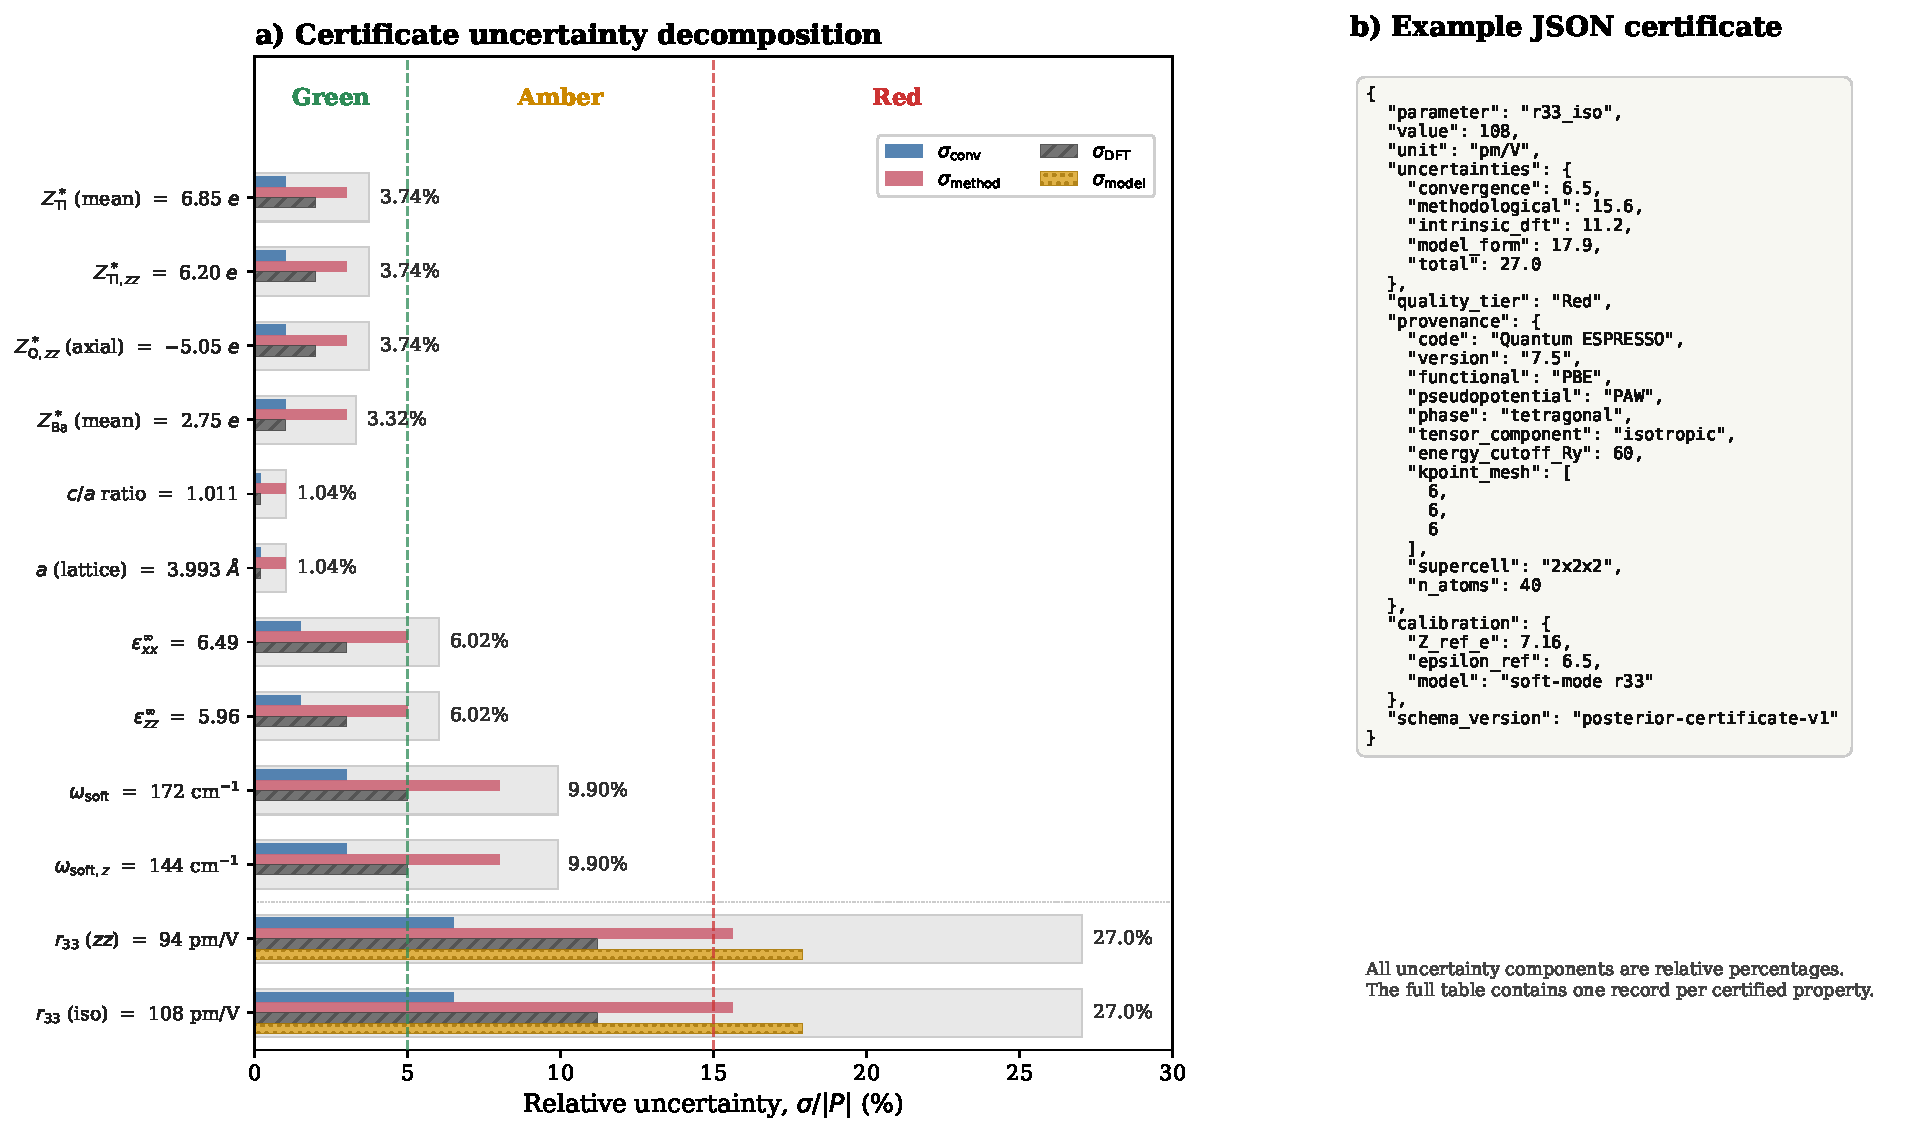
\includegraphics[width=\textwidth]{fig2_composite.pdf}
\caption{Posterior certificates from the BaTiO$_3$ $2\times2\times2$ 
supercell DFPT calculation (PBE/PAW, 60~Ry cutoff, $6\times6\times6$ k-point mesh). (a) Computed structural, dielectric, phonon, and electro-optic properties together with the decomposition of their relative uncertainties into convergence (blue), methodological (red), intrinsic DFT (dark gray), and model-form (gold) contributions. Light gray bars show the total relative uncertainty $\sigma_{\mathrm{total}}/|P|$. 
%Left: computed values. Right: uncertainty decomposition into convergence (blue), methodological (red), intrinsic DFT (dark gray, hatched), and model-form (gold, dotted, derived properties only) components; light gray bars show the quadrature total $\sigma_{\mathrm{total}}/|P|$.
Dashed 
lines at 5\% and 15\% mark Green/Amber and Amber/Red tier boundaries, respectively. The derived $r_{33}$ is 
reported in both $zz$ and isotropic tensor conventions, using 
literature-standard reference values ($Z^*_{\mathrm{ref}} = 7.16$~$e$, 
$\varepsilon_{\mathrm{ref}} = 6.5$); see Section~\ref{sec:library_update} 
for discussion of the convention dependence. (b) Example JSON representation of a posterior certificate, illustrating the structured metadata schema used to encode computed values, uncertainty decomposition, provenance information and quality-tier assignment. Further details are provided in Supplemental Material Section~S2.}
\label{fig:certificate_tiers}
\end{figure*}

\subsection{Certificate Generation}
\label{sec:cert_generation}

With the convergence and methodological components characterized, we can now 
assemble complete certificates for all 12 properties from a single DFPT
calculation. Figure~\ref{fig:certificate_tiers} shows the 12 
 certificates for the $2\times2\times2$ tetragonal BaTiO$_3$ supercell calculation (PBE/PAW DFPT  Quantum 
ESPRESSO 7.5 \cite{Giannozzi2009_QE}, 
60~Ry cutoff, $6\times6\times6$ k-point mesh). The certified quantities span structural, 
dielectric, phonon, and derived electro-optic properties, together with their 
uncertainty decomposition and quality tier assignment.


For the 10 directly computed properties, 
$\sigma_{\mathrm{model}} = 0$ and the certificates contain three active uncertainty
components. For the derived electro-optic response, however, all four uncertainty layers contribute significantly. The decomposition for $r_{33}$ includes: $\sigma_\conv = 6.5\%$ 
%(pure numerical convergence of the DFT inputs, propagated through the Jacobian); 
$\sigma_{\mathrm{DFT}} = 11.2\%$; 
%(propagated intrinsic exchange-correlation  errors of the input properties); 
$\sigma_\meth = 15.6\%$; 
%(propagated cross-functional spread)
and $\sigma_{\mathrm{model}} = 17.9\%$, combining to a total relative uncertainty of $27.0\%$ and placing the derived Pockels coefficient in the Red tier.
%(the phenomenological soft-mode approximation plus reference calibration uncertainty). 

The model-form contribution in the above reflects the limitations of the soft-mode approximation itself together with uncertainty in the reference calibration parameters. Veithen et al.\ \cite{Veithen2005} found that the soft-mode model reproduced approximately 80-90\% of the ionic electro-optic response in BaTiO$_3$, with the remaining discrepancy arising from electronic and multi-mode contributions. Combining this estimated 15\% approximation uncertainty with the 9.8\% calibration uncertainty gives $\sigma_{\mathrm{model}} = 17.9\%$. 
%the ionic contribution to within 10--20\%, with the discrepancy arising from electronic (clamped-ion) contributions and multi-mode coupling---with a 9.8\% calibration uncertainty, giving $\sigma_{\mathrm{model}} = \sqrt{15.0^2 + 9.8^2}\% = 17.9\%$. 
Similar soft-mode dominance has also been reported for LiNbO$_3$\cite{Veithen2004_PRL}, whereas PbTiO$_3$ shows dominant electronic contributions instead. 
%This 15\% approximation error is corroborated across materials: Veithen et al.\ \cite{Veithen2004_PRL} found comparable soft-mode dominance in LiNbO$_3$ ($\sim$80\% of ionic response) but not in PbTiO$_3$, where electronic contributions dominate. 

The resulting quality tier 
distribution (6 Green certificates, 4 Amber, 2 Red) is typical for well-converged 
DFPT calculations: structural and charge-response properties converge well, 
dielectric and phonon properties retain larger methodological sensitivity,  and derived electro-optic quantities inherit amplified uncertainty through the soft-mode dependence. 

\subsection{Library Update: Incorporating 2024--2025 Data}
\label{sec:library_update}

%The certificates in Fig.~\ref{fig:certificate_tiers} characterize a single PBE calculation. In practice, the certificate framework is designed to fuse multiple calculations: the single-calculation certificates ($r_{33} = 94$~pm/V in the $zz$ convention, $108$~pm/V isotropic, both at $\sigma_{\mathrm{total}} = 27.0\%$) become inputs to the inverse-variance--weighted library average. 
To test how single-calculation APECs fuse together as new calculations become available, we consider six additional entries from recent DFPT studies and compute the resulting fused inverse-variance-weighted  error estimates.  
PBEsol and PBE entries were included from the study by Amounas et al.\ \cite{Amounas2024} testing 24 exchange-correlation functionals 
in Quantum ESPRESSO for the spontaneous polarization and refractive indices 
of tetragonal BaTiO$_3$. 
%, finding $P_s$ values spanning 0.18--0.38~C/m$^2$ across functionals with the PBEsol result ($P_s = 0.26$~C/m$^2$) closest to experiment. 
 GGA+$U$ 
and hybrid functional optical properties at room temperature from the work by  Inerbaev et al.\ \cite{Inerbaev2025}, providing 
additional cross-checks on the dielectric response, were also included. Combined with our own 
DFPT results from Figure~\ref{fig:certificate_tiers}, these additions 
increase the library from 25 to 31 entries.

Building on the phase-aware partitioning introduced in Table \ref{tab:literature_library}, Table~\ref{tab:library_update} quantifies its effect 
on fused library averages and derived $r_{33}$. The unpartitioned library 
conflates cubic-phase and tetragonal-phase values for 
$Z^*_{\mathrm{Ti}}$ and mixes isotropic averages with $zz$~components for 
$\varepsilon^\infty$. When the tetragonal-phase PBE values are added 
without partitioning, the uncertainty in $\varepsilon^\infty$  \emph{widens} 
by 60\%, indicating a data curation problem, not a solution to it. 
Partitioning by phase and tensor component resolves the discrepancies 
and yields consistent fused estimates.

\begin{table*}
\centering
\caption{Effect of phase-aware library partitioning on key parameters 
and derived $r_{33}$. ``Unpartitioned'' averages all entries regardless of 
phase; ``Phase-filtered'' averages within consistent (phase, component) 
subsets. The $r_{33}$ uncertainties include propagated input uncertainties 
and 17.9\% model-form uncertainty from the soft-mode approximation. The final column 
shows the relative uncertainty $\sigma_\text{rel}$ calculated from the standard deviation reported for the $r_{33}$ values, showing the reduction obtained through library fusion relative to the single-calculation certificates of Figure \ref{fig:certificate_tiers}.}
\label{tab:library_update}
\begin{tabular}{lccccc}
\toprule
Input convention & $Z^*_{\mathrm{Ti}}$ ($e$) & $\varepsilon^\infty$ & $\omega_{\mathrm{soft}}$ (cm$^{-1}$) & $r_{33}$ (pm/V) & $\sigma_{\mathrm{rel}}$ \\
\midrule
Unpartitioned library & \;\;$7.29 \pm 0.28$ \;\; & $6.51 \pm 0.40$ & $176 \pm 6$ & $114 \pm 22$ & 19\% \\
Tetragonal, isotropic avg & \;\;$6.85 \pm 0.20$ \;\;& $6.31 \pm 0.25$ & $172 \pm 6$ & $108 \pm 22$ & 20\% \\
Tetragonal, $zz$ only & \;\;$6.20 \pm 0.20$ \;\;& $5.96 \pm 0.18$ & $172 \pm 6$ & $94 \pm 19$ & 20\% \\
Single calc, $zz$ (Figure~\ref{fig:certificate_tiers}) & $6.20$ & $5.96$ & $172$ & $94 \pm 25$ & 27\% \\
Single calc, iso (Figure~\ref{fig:certificate_tiers}) & $6.85$ & $6.32$ & $172$ & $108 \pm 29$ & 27\% \\
\midrule
Experiment (bulk, 300~K) & --- & --- & --- & $105 \pm 15$ & 14\% \\
\bottomrule
\end{tabular}
\end{table*}

The impact on the derived $r_{33}$ is substantial. The unpartitioned library 
average ($r_{33} = 114 \pm 22$~pm/V) is inflated primarily because it draws 
$Z^*_{\mathrm{Ti}}$ predominantly from cubic-phase DFPT 
studies \cite{Ghosez1998_BEC,Zhong1994_BTO,Veithen2005} where  $Z^*_{zz} = 7.3$~$e$. In the tetragonal phase, the 
 corresponding component drops to 6.20~$e$ due to the ferroelectric distortion. 
Since $r_{33} \propto Z^{*2}$, this difference alone increases the 
fused electro-optic response by  $(7.29/6.85)^2 \approx 1.13$.

When tetragonal-phase isotropic averages are used consistently 
($Z^*_{\mathrm{Ti}} = 6.85$~$e$, $\varepsilon^\infty = 6.31$, 
$\omega_{\mathrm{soft}} = 172$~cm$^{-1}$), the model gives 
$r_{33} = 108$~pm/V, within 3\% of the bulk experimental value of 
Zgonik et al.\ ($105 \pm 15$~pm/V). The agreement indicates that the phase-consistent fused library provides a physically realistic description of the electro-optic response. Since the experimental measurement provides an averaged bulk response, comparison with the isotropic convention is more appropriate than comparison with a single tensor component. The $zz$-component 
value ($r_{33} = 94$~pm/V) is instead the relevant prediction for a 
single-domain, $z$-polarized device geometry.

The single-calculation certificates in Figure ~\ref{fig:certificate_tiers} are fully consistent with the corresponding fused library values.  
The $zz$-only certificate gives $r_{33} = 94 \pm 25$~pm/V, 
matching the tetragonal $zz$ library average ($94 \pm 19$~pm/V), whereas 
the isotropic certificate gives $r_{33} = 108 \pm 29$~pm/V, matching 
the tetragonal isotropic library average ($108 \pm 22$~pm/V). The consistency 
between single-calculation and library-fused values validates the extraction pipeline within the 
soft-mode model. The 14\% difference between $zz$ and isotropic values 
($94$ vs $108$~pm/V) quantifies the impact of tensor averaging and 
reinforces the need to track phase and tensor-convention metadata explicitly. 

Beyond resolving convention ambiguities, library fusion reduces the uncertainty of the derived electro-optic response.
The single calculation certificates carry a total relative uncertainty of  
 27\%, whereas fusing with the phase-filtered literature reduces this 
to $\sim$20\%. This improvement is primarily driven by 
a reduction in methodological uncertainty as information from multiple functionals and implementations is combined. The absolute uncertainty bars also shrink, from 
$\pm 25$ to $\pm 19$~pm/V for the $zz$ convention, from $\pm 29$ to 
$\pm 22$~pm/V for the isotropic convention. 

Data fusion does not reduce the 
model-form contribution ($\sigma_{\mathrm{model}} = 17.9\%$), which sets an 
irreducible floor on the achievable $r_{33}$ uncertainty within the 
soft-mode approximation. Further improvement would require either  a more accurate 
phenomenological description or full \emph{ab initio} electro-optic tensor calculation. 
The reduction in uncertainty upon fusion from 27\% to 20\%  illustrates how  the 
certificate framework can be leveraged to not merely \emph{track} uncertainty but actively 
\emph{reduce} it through principled data combination.

A leave-one-out calibration test of the phase/component-consistent subsets of the BaTiO$_3$ literature subsets is presented in Supplemental Material Section~S3.7. The test yielded a mean standardized residual of -0.02, a root-mean-square residual of 1.05 and empirical coverage close to the expected 68\% and 95\% confidence levels. These results suggest that the present certificate library is reasonably calibrated and neither strongly over- nor under-confident.





%\subsection{Posterior Calibration Check}
%\label{sec:calibration_check}

%As an initial calibration test, we performed a leave-one-out posterior predictive check on the phase/component-consistent subsets of the BaTiO$_3$ literature library. For each subset with at least three computational entries ($\omega_{\mathrm{soft}}$, $Z^*_{\mathrm{Ti},zz}$, $P_s$, and lattice parameter $a$), one entry was held out, the remaining entries were fused by inverse-variance weighting, and the held-out residual was standardized as
%\begin{equation}
%    z_i =
%    \frac{P_i - \hat{P}_{-i}}
%    {\sqrt{\sigma_i^2 + \sigma_{-i}^2}} .
%    \label{eq:loo_calibration}
%\end{equation}
%If the reported uncertainties are calibrated and the entries are approximately exchangeable within each subset, these residuals should follow a standard normal distribution. Across 15 leave-one-out residuals, the mean $z$ score is $-0.02$, the root-mean-square $z$ score is 1.05, and the pooled reduced $\chi^2$ is 1.10. The empirical coverage is 73\% for $|z| < 1$ (68\% expected) and 93\% for $|z| < 1.96$ (95\% expected). The room-temperature bulk experimental comparison for the fused isotropic $r_{33}$ gives $z = 0.11$ relative to the Zgonik et al.\ \cite{Zgonik1994} reference value. These statistics are not a substitute for a large benchmark campaign, but they show that the present certificate library is not grossly over- or under-confident at the scale probed by the available data.

%\begin{figure*}
%    \centering
%    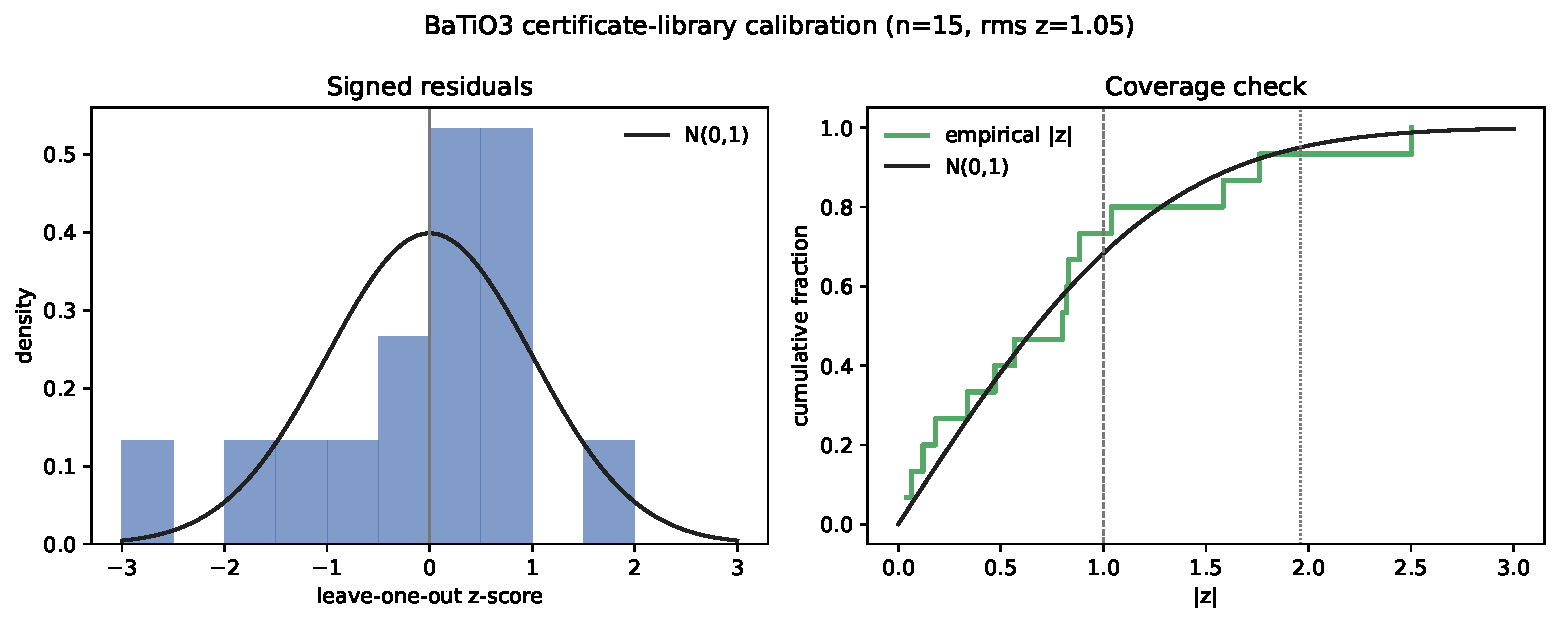
\includegraphics[width=\textwidth]{fig3_calibration_check.pdf}
%    \caption{Leave-one-out calibration check for the BaTiO$_3$ certificate    library. The left panel shows standardized residuals for held-out    literature entries relative to inverse-variance fusion of the remaining    entries in the same phase/component subset. The right panel compares the    empirical coverage of $|z|$ with the standard-normal expectation.}
%    \label{fig:calibration_check}
%\end{figure*}

%\subsection{Propagation to Device Metrics}



%%%%%%%%%%%%%%%%%%%%%%%%%%%%%%%%%%%%%%%%%%%%%%%%%%%%%%%%%%%%%%%%%%%%%%%%%%%%%%%
\section{Discussion}
\label{sec:discussion}
%%%%%%%%%%%%%%%%%%%%%%%%%%%%%%%%%%%%%%%%%%%%%%%%%%%%%%%%%%%%%%%%%%%%%%%%%%%%%%%

The results presented in the  BaTiO$_3$ case study illustrate several distinct roles of APECs. First, APECs help quantify the uncertainty associated with individual DFT-computed and derived quantities with decomposition into convergence, methodological, intrinsic DFT, and model-form contributions. 
Second, they enable uncertainty-aware fusion of heterogeneous data sources, allowing literature values, database entries, and new calculations to be combined in a consistent manner. 
Third, they propagate uncertainty through nonlinear physical relationships, making explicit how uncertainties in computed descriptors influence derived observables. 
Finally, the uncertainty decomposition helps identify where additional information can most effectively improve predictions. In the present example, numerical convergence contributes relatively little to the total uncertainty of the electro-optic response, whereas methodological and model-form contributions dominate. Consequently, additional convergence studies are expected to yield only marginal improvements in uncertainty. In contrast, new cross-functional calculations, direct electro-optic tensor calculations, and improved calibration data would reduce uncertainty more substantially. These uses make  uncertainty quantification  an effective tool for guiding further computational and experimental effort.

\subsection{Applicability, Assumptions, Limitations}

Posterior certification is most valuable when uncertainty influences scientific or applicability decisions. The BaTiO$_3$ study presented here highlights two particularly important situations: the aggregation of heterogeneous datasets, and the propagation of uncertainty through nonlinear physical models.  In the former, provenance-aware fusion revealed phase and tensor-component inconsistencies that would have remained hidden with a conventional literature average. In the latter, the inverse-square dependence of r$_{33}$ on the soft-mode frequency amplified modest uncertainties in  $\omega_{\text{soft}}$ into substantially larger uncertainties in the derived electro-optic response. Similar challenges arise throughout computational materials science whenever results from multiple sources must be combined, such as machine learned or fitted multiscale approaches \cite{Henderson2023}, or when derived quantities depend sensitively on underlying DFT observables. 
 
%First, when data heterogeneity is high---that is, when results from multiple groups, codes, or parameter choices must be combined. Second, when uncertainty amplification exists in the physical model, as occurs for any derived quantity with nonlinear dependence on DFT properties (the $r \propto \omega^{-2}$ relationship being a paradigmatic example). Third, when the stakes of downstream decisions are significant, whether in screening with asymmetric false-positive/negative costs or in quantitative device design. And fourth, when ML calibration matters, as in active learning or Bayesian optimization workflows that rely on trustworthy uncertainty estimates.

%Conversely, for well-established properties computed with standard methods on familiar material classes, the overhead of full certification may not be justified. The framework is designed to scale gracefully: heuristic estimates and tier downgrading allow partial certification when full convergence data is unavailable.

%\subsection{Limitations}
%\label{sec:limitations}

The method rests on several assumptions and approximations whose impact should be 
understood before the certificates are used in downstream applications. 
These include the assumption of independent uncertainty contributions, the scope of modeled 
uncertainty, the availability of benchmark data for estimating methodological error, and the recursive nature 
of surrogate model uncertainty.

The independence assumption underlying the variance decomposition 
(Equation~\ref{eq:error_model}) is the most significant approximation. As shown 
in Section~\ref{sec:decomposition}, a two-functional (LDA/PBE) covariance 
estimate reveals that the cross-functional shifts in $Z^*$, 
$\varepsilon^\infty$, and $\omega_{\mathrm{soft}}$ partially cancel in 
$r_{33}$, making independence conservative for this observable by a 
substantial factor. However, this estimate is based on only two functionals 
and assumes the cancellation pattern generalizes across materials. A more rigorous assessment would require convergence studies that track all three quantities simultaneously, allowing covarience data to be determined directly rather than inferred from cross-functional trends. 
 The covariance terms in 
Equation~\ref{eq:linear_prop} provide the formal mechanism for incorporating 
such data once available.

The framework quantifies only sources of uncertainty explicitly represented in the certificate. Unmodeled 
effects such as code errors, incorrect inputs, or missing physics are not 
captured by the four-component decomposition. However, deviations between 
single-calculation certificates and aggregated literature data can provide useful diagnostic information. In the present work,  the discrepancy between the single-calculation and 
library-fused $r_{33}$ highlighted a metadata labeling error in the reference data:  The addition of new data increased rather than decreased the uncertainty in $\varepsilon_\infty$, indicating that physically distinct quantities were being combined within the same average. The issue was resolved manually. The certificate framework does not diagnose such 
errors automatically, but it creates the conditions under which they 
become visible. 

Similarly, the method helps identify  inconsistencies in aggregated datasets, for example when quantities from different crystallographic phases or tensor conventions are combined inappropriately. In the present case, identifying the source of discrepancy required human inspection of the metadata. However, the phase, tensor-component and functional provenance tags can also provide the information needed for automated detection. Without explicit provenance tracking, phase and component conflations would be invisible within a simple literature average.

Accurate estimation of $\sigma_\meth$ and $\sigma_{\mathrm{DFT}}$ requires 
benchmark data. For novel properties or material classes where such data is 
unavailable, the method must fall back on cross-functional spread as a proxy, 
which provides a lower bound on the true methodological uncertainty.

Finally, full convergence studies multiply computational cost, and our surrogate 
models for estimating $\sigma_\conv$ from single calculations introduce their 
own uncertainty. In principle, the framework is recursive: the surrogates 
themselves are candidates for certification, and their fitting error should 
propagate as a second-order contribution into every certificate they generate. 
This meta-uncertainty is currently neglected but should be quantified as the 
surrogate models mature. The trade-off between certification fidelity and 
computational budget is application-dependent.

\subsection{Scope of the Current Certificate}

The present certificates describe bulk tetragonal BaTiO$_3$ and quantify uncertainty within the physical and computational assumptions of the underlying model. Important sources of electro-optic enhancement in experimental devices, including epitaxial strain, domain engineering, finite-temperature effects,  and phase stability, are not explicitly represented in the current form. 

Much current interest in BaTiO$_3$ has focused on strain-induced enhancement of the electro-optic coefficient for a variety of applications. Among these studies, are thin-film measurements.  Reynaud et al.\ \cite{Reynaud2025} report an effective Pockels coefficient exceeding 550~pm/V in 150~nm epitaxial films on Si. This value is a factor of $\sim$$5\times$ above the bulk value, due to domain-structure optimizations not captured in bulk calculations. Suceava et al.\ \cite{Suceava2025} achieve $r_{33} = 2516 \pm 100$~pm/V at 5~K in strain-stabilized metastable films, reflecting a monoclinic phase where $\omega_{\mathrm{soft}}$ is further suppressed by epitaxial strain. These measurements highlight physical mechanisms that are not included in the present bulk certificate, including domain structure, strain coupling, temperature dependence and phase stability. Extending the certification approach to incorporate these additional sources of variability will allow their contributions and associated uncertainties to be quantified, and are the natural next step in the APECs framework.

\subsection{Extension and Adoption}

The certified {\em bulk} $r_{33}$ is not the end of the uncertainty chain. For device design, performance metrics such as the effective electro-optic coefficient $r_{\mathrm{eff}}$ and the half-wave voltage--length product $V_\pi L = \frac{\lambda d}{2 n^3 r_{\mathrm{eff}} \Gamma}$ (where $\lambda$ is the wavelength, $d$ is the electrode gap, $n$ is the refractive index, and $\Gamma$ is the optical--RF field overlap \cite{Wooten2000,Reed2010,Wang2018_LN_thin}) are obtained through a sequence of additional modeling steps that introduce their own uncertainty sources. Table \ref{tab:propagation} illustrates this concept using a representative propagation chain from the certified bulk BaTiO$3$ response ($r_{33}=108 \pm 22$ pm/V) to derived effective material parameters and ultimately device-level metrics. Library fusion improves the starting point for this propagation by reducing the uncertainty in the bulk electro-optic response from 27\% for a single calculation to approximately 20\% for the fused library value, approaching the model-form uncertainty floor imposed by the soft-mode approximation. The table illustrates two important points: (i) Downstream calculations benefit directly from improvements in the underlying materials data, and (ii) Each additional stage from bulk material properties to device-level metrics contributes new uncertainty that must be quantified and propagated alongside the underlying DFT uncertainty. Crucially, the chain structure makes the dominant uncertainty source visible at each stage. In the present example, uncertainty in the DFT-derived electro-optic response remains one of the largest contributors even at the device level, but future implementations could incorporate additional uncertainties arising from domain structure, strain state, fabrication tolerances, optical mode confinement, and operating temperature within the same framework.


%Table~\ref{tab:propagation} traces uncertainty through the device modeling chain, showing both the single-calculation certificate and the library-fused value at the Property stage. The fusion benefit propagates through all downstream stages, reducing device-level uncertainty from $\sim$32\% to $\sim$24\%.

%Table~\ref{tab:propagation} shows both the single-calculation and library-fused $r_{33}$ to make the fusion benefit visible within the chain: library fusion compresses the Property-stage uncertainty from 27\% to 20\%, approaching the irreducible model-form floor ($\sim$18\%). The downstream stages propagate from this improved baseline: microstructure averaging introduces $\sim$10\% additional uncertainty from domain orientation statistics \cite{Reynaud2025}, and the device model contributes $\sim$5\% from geometric and overlap integral uncertainties, giving $\sim$24\% at the device level rather than $\sim$32\% without fusion. Crucially, the chain structure makes the dominant uncertainty source visible at each stage: DFT-level uncertainty dominates even at the device level, confirming that certification at the source has the greatest leverage. The sensitivity (gain) factors between stages---$\times 2$ for soft-mode amplification, $\sim \times 1$ for downstream stages---quantify exactly where uncertainty reduction efforts will have the most impact. The current propagation chain does not capture optical propagation loss, which Kim and Demkov \cite{Kim2025_loss} have shown to be dominated by non-absorptive scattering at ferroelectric domain walls in BTO waveguides. This is a known unmodeled effect: the certificate framework as presented tracks uncertainty in $r_{\mathrm{eff}}$ and $V_\pi L$ but not in insertion loss, which enters the device figure of merit independently. Extending the certificate schema to include loss parameters---potentially calibrated against low-loss demonstrations such as the high-$Q$ ring resonators of Raju et al.\ \cite{Raju2025}---is a natural direction for future work. The DFT-derived $r_{33}$ remains the dominant uncertainty source throughout the modulation-efficiency chain.

\begin{table*}
\centering
\caption{Illustrative propagation of certified uncertainties from bulk material to device-level metrics. Each row represents a certificate-generating stage. The DFT and Property stages use the uncertainty decomposition developed in this work and summarized in   Figure \ref{fig:certificate_tiers}; the Effective and Device stages employ representative uncertainty estimates to illustrate how additional modeling stages can be incorporated in the same framework. }
\label{tab:propagation}
\begin{tabular}{llcc}
\toprule
Stage & Quantity & Value & Rel.\ uncertainty \\
\midrule
DFT & $\omega_{\mathrm{soft}}$ & 172 cm$^{-1}$ & 10\% \\
$\downarrow$ ($\times 2$ amplification) & & & \\
Property (single calc) & $r_{33}$ ($zz$) & 94 pm/V & 27\% \\
Property (library-fused) & $r_{33}$ ($zz$) & 94 pm/V & 20\% \\
\midrule
\multicolumn{4}{l}{\textit{Downstream stages (to be certified):}} \\
$\downarrow$ (microstructure averaging) & & & \\
Effective & $r_{\mathrm{eff}}$ & $\sim$40 pm/V & $\sim$22\% \\
$\downarrow$ (device model) & & & \\
Device & $V_\pi L$ & $\sim$2.5 V$\cdot$cm & $\sim$24\% \\
\bottomrule
\end{tabular}
\end{table*}

The structured nature of the certificate metadata also creates opportunities beyond uncertainty quantification for individual calculations. Recent work in materials informatics has highlighted the importance of uncertainty-aware machine learning, particularly when training models on heterogeneous datasets assembled from multiple computational and experimental sources \cite{Kendall2017,Nix1994,Guo2017_calibration,Kuleshov2018,Tran2018_active}. The uncertainty estimates associated with individual certificates provide a natural mechanism for incorporating data quality into model development, whether through inverse-variance weighting, calibration analysis, or heteroscedastic learning approaches that explicitly distinguish between data uncertainty and model uncertainty. More broadly, certificate metadata could enable uncertainty-aware aggregation and filtering of large materials datasets. Evaluating these ideas in graph neural network and foundation-model workflows trained on heterogeneous materials databases represents an interesting direction for future work \cite{Schutt2018_SchNet,Chen2022_M3GNet,Batatia2022_MACE}.
%Community adoption requires action at several levels. At the code level, major DFT packages (VASP, QE, FHI-aims) could add optional certificate output with minimal changes---primarily metadata collection and JSON serialization. At the database level, Materials Project, AFLOW, and JARVIS APIs could extend their schemas to accept and serve certificate fields, enabling filtering by quality tier. Systematic benchmark campaigns across material classes are needed to parameterize the surrogate convergence models (Supplemental Material, Table~S3). At the machine learning level, the certificate schema exposes three interface points: inverse-variance loss weighting ($\mathcal{L} \propto \sum_i (y_i - \hat{y}_i)^2 / \sigma_i^2$) to focus model capacity on high-quality data, heteroscedastic architectures that separate irreducible label noise from learned epistemic uncertainty \cite{Kendall2017,Nix1994}, and calibration validation using certificates as ground-truth uncertainty targets \cite{Guo2017_calibration,Kuleshov2018,Tran2018_active}. These are interface specifications; systematic evaluation on graph neural networks \cite{Schutt2018_SchNet,Chen2022_M3GNet,Batatia2022_MACE} trained on heterogeneous database aggregates is the subject of ongoing work. Finally, a community workshop or working group could establish consensus on tier thresholds, schema versions, and best practices for certificate-aware analysis.

%%%%%%%%%%%%%%%%%%%%%%%%%%%%%%%%%%%%%%%%%%%%%%%%%%%%%%%%%%%%%%%%%%%%%%%%%%%%%%%
\section{Conclusion}
\label{sec:conclusion}
%%%%%%%%%%%%%%%%%%%%%%%%%%%%%%%%%%%%%%%%%%%%%%%%%%%%%%%%%%%%%%%%%%%%%%%%%%%%%%%

We have introduced A Posteriori Error Certificates (APECs), a methodology for attaching quantitative uncertainty estimates and provenance metadata to DFT-calculated values and the properties derived from them.  By decomposing  uncertainty into convergence, methodological, intrinsic DFT, 
and model-form components, the method provides a structured description of the confidence associated with computed materials properties, enables uncertainty propagation through derived quantities, supports the consistent fusion of heterogeneous data, and assigns Green, Amber and Red quality tiers to data based on overall uncertainty. 

The BaTiO$_3$ application of the APECs framework   demonstrates that 
soft-mode amplification pushes the derived Pockels coefficient to Red 
tier ($\sigma_{\mathrm{total}} = 27.0\%$) even when the underlying DFT-calculated 
properties are Green or Amber. Phase-aware partitioning of literature 
data resolved inconsistencies arising from mixing cubic and tetragonal data and reduced the uncertainty in the library-fused electro-optic response to 20\%. Although demonstrated here for the soft-mode electro-optic response of BaTiO$_3$, the method is independent of the underlying electronic-structure method or property. More broadly, APECs provide a  basis for uncertainty-aware computational materials science, allowing computed properties to be compared, combined, and used systematically in databases, multiscale models and future data-driven materials design.

%The thin-film  discrepancy ($5$--$22\times$ above bulk) quantifies the modeling gap that microstructure and strain stages of the propagation chain must close.

%Several open problems define the path forward. First, the heuristic cross-functional covariance estimate presented here (Section~\ref{sec:decomposition}) should be validated against empirical convergence-level covariance data from systematic parameter sweeps; comparing the two will establish whether the partial cancellation observed in BaTiO$_3$ is transferable to other perovskites or is material-specific. Second, the surrogate convergence models (Supplemental Material, Table~S3) require systematic fitting against dedicated benchmark datasets across material classes. Third, extending the propagation chain from bulk DFT through domain microstructure, strain coupling, and device geometry would connect the certificate framework to multi-physics digital twin pipelines. Fourth, quantifying whether inverse-variance loss weighting and certificate-derived aleatoric noise floors improve generalization in graph neural network potentials trained on heterogeneous database aggregates would establish the practical value of certificate-aware machine learning for materials prediction.

%%%%%%%%%%%%%%%%%%%%%%%%%%%%%%%%%%%%%%%%%%%%%%%%%%%%%%%%%%%%%%%%%%%%%%%%%%%%%%%
\section{Methods: A Posteriori Error Certificates}
\label{sec:methods}
%%%%%%%%%%%%%%%%%%%%%%%%%%%%%%%%%%%%%%%%%%%%%%%%%%%%%%%%%%%%%%%%%%%%%%%%%%%%%%%

\subsection{Sources of Uncertainty in DFT}
\label{sec:bg_sources}

The output of a DFT calculation \cite{Hohenberg1964,KohnSham1965} depends on 
a variety of choices, each introducing distinct sources of error. These errors can be roughly grouped in three categories: intrinsic, methodological, and convergence. 

 \emph{Convergence} is sought in materials' DFT calculations at several points. Plane-wave DFT requires truncation of the 
basis set at a finite energy cutoff $\Ecut$, sampling of the Brillouin zone 
on a discrete $k$-point mesh, and iterative solution of the Kohn--Sham 
equations to a finite self-consistency threshold 
\cite{Kresse1996_VASP,Giannozzi2009_QE,Blum2009_FHIaims}. These parameters must be converged for each property and material system, 
and the degree to which a given calculation has achieved convergence is often 
not reported in online data.

At the \emph{methodological} level, the choice of DFT code, exchange-correlation 
functional, basis set and pseudopotential, all introduce systematic errors that vary by property and material class
\cite{Perdew2001_Jacobs_Ladder,Mardirossian2017,Medvedev2017,Sun2015_SCAN,Furness2020_r2SCAN}. To illustrate, we include representative bias statistics, ranging from $<$1\% for 
lattice constants with the PBEsol or SCAN functionals to up to  $\sim$40\% errors for band gaps using 
semilocal functionals, in Supplemental Material Table~S1.

At the \emph{intrinsic} level, even with perfect convergence and an ideal 
functional, Kohn--Sham DFT has fundamental limitations: strong correlation 
%(an issue particularly for systems such as Mott insulators or heavy fermions) 
\cite{Georges1996_DMFT,Anisimov1997}, 
long-range dispersion when not considered explicitly, the 
fundamental band gap problem of DFT \cite{Perdew1983,Sham1983}, spin--orbit 
coupling in heavy elements, and finite-temperature effects
\cite{Cohen2008,Becke2014,Grimme2010_D3,Klimes2012_vdW}.
These constitute an irreducible floor on achievable accuracy within the DFT 
framework.

The certificate framework was presented conceptually in the preceding sections. Below, we introduce mathematically each uncertainty component and the estimation procedures used to build APECs.
%The certificate framework proposed here aims to address several of these concerns: (i)  uncertainty is divided into physically meaningful components (convergence, methodological, intrinsic, and model-form); (ii) the framework works with any functional and any code, including retrospective application to existing databases; (iii) interpretable quality classes are assigned for filtering and stratification; (iv)  uncertainty is propagated through derived quantities and multi-stage workflows; and (v) it iscompatible with automated pipelines and machine learning integration. The posterior error certificate framework is described in the following section.



\subsection{Certificate Structure}
\label{sec:cert_structure}

A posterior error certificate $\cert[P]$ attaches an uncertainty estimate to a computed property $\hat{P}$ as a metadata object. It is ``posterior'' in the sense that it can be evaluated after the calculation, using 
the computational output, convergence behavior, 
and available benchmark data. Formally:
\begin{equation}
    \cert[P] = \left\{ \hat{P}, \, \sigma_\conv, \, \sigma_\meth, \, 
    \sigma_{\mathrm{DFT}}, \, \sigma_{\mathrm{model}}, \, \sigma_{\mathrm{total}}, \, 
    \tau, \, \Pi \right\}
    \label{eq:certificate}
\end{equation}
where four uncertainty 
components are included for convergence ($\sigma_\conv$), methodology ($\sigma_\meth$), 
intrinsic DFT error ($\sigma_{\mathrm{DFT}}$), and, for derived quantities,  
model-form error ($\sigma_{\mathrm{model}}$). The uncertainty components are assumed to be independent in the first approximation; details on considering correlations are provided in Supplemental Material Section~S1.1. The total uncertainty is taken as the quadrature sum (see Equation \ref{eq:sigma_sum}).
The certificate also includes the quality tier estimate
$\tau \in \{\text{red}, \text{amber}, \text{green}\}$; and provenance 
metadata $\Pi$ recording the code, version, functional, pseudopotential, 
all convergence parameters, the 
crystallographic phase and tensor convention used in the calculation. 
Tracking this information specifically is essential when combining literature data, since quantities such as Born effective charges and dielectric tensor can differ substantially between cubic and tetragonal phases and between $zz$ and isotropic tensor averages.  

For properties computed directly from DFT, 
$\sigma_{\mathrm{model}} = 0$. For derived properties (e.g., the soft-mode expression for $r_{33}$), 
$\sigma_{\mathrm{model}}$ captures the approximation error of that model 
and is nonzero. Implementation details are provided in Supplemental Material Sections~S2.2--S2.3 and qff package documentation. 
%The full JSON schema specification and a reference implementation of the data aggregation pipeline are provided in the Supplemental  Material~\footnote{See Supplemental Material at [URL will be inserted by  publisher] for extended formalism (hierarchical Bayesian fusion, Monte Carlo propagation, convergence estimators), the JSON certificate schema, supporting data tables (functional bias statistics, cross-functional soft-mode comparison, convergence model parameters, heuristic estimates), the complete 31-entry BaTiO$_3$ literature library with phase metadata, certificate data for all 12 properties, and the extraction case study walkthrough.} and in the qff package documentation.

\subsection{Error Model and Uncertainty Decomposition}
\label{sec:decomposition}

We model the computed or derived property 
as \cite{JCGM2008_GUM}
\begin{equation}
    P_{\mathrm{computed}} = P_{\mathrm{true}} + \epsilon_\conv + \epsilon_\meth + \epsilon_{\mathrm{DFT}} + \epsilon_{\mathrm{model}}
    \label{eq:error_model}
\end{equation}

The four error terms are assumed to be independent. This is 
the central approximation of the method and deserves explicit 
justification. 
The convergence error $\epsilon_\conv$ is dominated by basis set truncation 
and $k$-point sampling -- numerical parameters that are largely 
functional-independent. The methodological error $\epsilon_\meth$ reflects 
the choice of exchange-correlation functional, pseudopotential type, and 
related recipe decisions. The intrinsic DFT error $\epsilon_{\mathrm{DFT}}$ 
captures limitations shared by all standard functionals (e.g., 
self-interaction, static correlation). 

In practice, correlations exist: 
a functional that overbinds will systematically stiffen phonons, coupling 
$\epsilon_\meth$ to $\epsilon_{\mathrm{DFT}}$. We proceed with the 
independence assumption as a zeroth-order baseline but can estimate its 
impact from existing data. Comparing LDA and PBE values in the compiled literature 
library (Supplemental Material Table~S5), the three quantities entering the soft-mode expression for $r_{33}$ shift systematically with the choice of functional. PBE gives slightly larger Born effective charges ($+5\%$) and dielectric constants ($+8\%$) than LDA, while the soft-mode frequency changes comparatively little.  Because contributions from $Z^*$ and $\varepsilon^\infty$ enter $r_{33} \propto 
Z^{*2}/(\varepsilon \omega^2)$ with opposite signs, these shifts partially cancel, reducing the net variation in the derived property: the net cross-functional shift 
in $r_{33}$ is only $\sim$2\%, compared to the $\sim$13\% expected from the independent 
quadrature of the individual uncertainties. 

This confirms that the independence  assumption is conservative for $r_{33}$, since it overestimates the methodological component of the $r_{33}$ uncertainty. We retain the conservative estimate as the default because (i) the present comparison is based on only two functionals, exaggerating the cancellation effect and (ii) this cancellation is specific to 
%for two reasons: first, the two-functional estimate is degenerate ($N = 2$ forces $|\rho| = 1$, overstating the cancellation); 
%second, the cancellation is specific to 
$r_{33}$. Other quantities may instead show reinforcing correlations. When sufficient material-specific data is available, covariance terms can be included specifically.
%observable-specific---$Z^*$ and $\varepsilon^\infty$ happen to enter $r_{33}$ with opposite signs, but other derived quantities may see reinforcing rather than canceling correlations. A general-purpose framework should default to the conservative bound and allow tightening when material-specific covariance data is available.
Alternatively, a more reliable estimate of the covariance could be obtained by systematically varying numerical parameters while tracking the resulting changes in 
$\omega_{\mathrm{soft}}$, $Z^*$, and $\varepsilon^\infty$  (See Section~\ref{sec:limitations}).

\subsubsection{Convergence Uncertainty ($\sigma_\conv$)}

Convergence error arises from finite computational 
parameters \cite{Payne1992}. For plane-wave DFT, the three dominant 
contributions to this are (i) basis set truncation, which decays exponentially with 
cutoff energy,
\begin{equation}
    \epsilon_{\Ecut}(E) = A_E \exp\left(-E / E_0\right);
    \label{eq:cutoff_error}
\end{equation}
(ii) Brillouin zone integration, which follows a power law in the number of 
$k$-points \cite{Wisesa2016,Monkhorst1976},
\begin{equation}
    \epsilon_k(\Nk) = B / \Nk^{\alpha},
    \label{eq:kpoint_error}
\end{equation}
where $\alpha \approx 1$ for metals and $\alpha \approx 2$ for insulators; and (iii) 
 incomplete self-consistency, arising from residual changes in the electron density at the end of the SCF cycle.
 %which contributes through the sensitivity of the property to the residual density at the final SCF iteration. 
 
The total convergence uncertainty is the quadrature sum of all 
contributions \cite{JCGM2008_GUM}:
\begin{equation}
    \sigma_\conv^2 = \sigma_{\Ecut}^2 + \sigma_k^2 + \sigma_{\mathrm{SCF}}^2 
    + \sigma_{\mathrm{FFT}}^2 + \cdots
    \label{eq:total_convergence}
\end{equation}
where additional terms such as FFT grid density, augmentation charge cutoff, Fermi 
smearing width, etc., are included when relevant. Details of the individual uncertainty estimates are provided in the Supporting  Information.

\subsubsection{Methodological Uncertainty ($\sigma_\meth$)}

Different computational ``recipes'', a specific combination of functional, 
pseudopotential \cite{Blochl1994_PAW,Garrity2014_GBRV}, and code, give 
systematically different results \cite{Lejaeghere2014}. We model 
each recipe as producing an estimate biased by $\beta_{\mathrm{recipe}}$:
\begin{equation}
    P_{\mathrm{recipe}} = P_{\mathrm{true}} + \beta_{\mathrm{recipe}} + \epsilon
    \label{eq:recipe_bias}
\end{equation}

When reference data exists from experiment or high-level theory (CCSD(T), DMC), 
biases can be estimated empirically:
\begin{equation}
    \hat{\beta}_{\xc} = \frac{1}{N_{\mathrm{ref}}} \sum_{i=1}^{N_{\mathrm{ref}}} 
    \left( P_{\xc,i} - P_{\mathrm{ref},i} \right)
    \label{eq:bias_estimate}
\end{equation}

For new chemistry, new materials or properties without benchmarks, the methodological 
uncertainty is estimated from the spread across available methods:
\begin{equation}
    \sigma_\meth^2 \approx \mathrm{Var}_{\mathrm{recipes}}[P_{\mathrm{recipe}}]
    = \frac{1}{M-1} \sum_{j=1}^{M} (P_j - \bar{P})^2
    \label{eq:method_spread}
\end{equation}

\subsubsection{Intrinsic DFT Uncertainty ($\sigma_{\mathrm{DFT}}$)}

We estimate $\sigma_{\mathrm{DFT}}$ from the residual spread relative to reference data after correcting systematic biases: 
\cite{Pernot2015,Pernot2020}:
\begin{equation}
    \sigma_{\mathrm{DFT}}^2 = \frac{1}{N_{\mathrm{ref}}} \sum_i 
    \left( P_{\xc,i} - \hat{\beta}_{\xc} - P_{\mathrm{ref},i} \right)^2
    \label{eq:intrinsic_dft}
\end{equation}

\subsubsection{Model-Form Uncertainty ($\sigma_{\mathrm{model}}$)}

%When a property is not computed directly from DFT but derived through a phenomenological model---for example, $r_{33}$ via the Johnston--Kaminow soft-mode relation---the model itself introduces approximation error that is conceptually distinct from the exchange-correlation limitations captured by 
For quantities derived from DFT-computed inputs, the model relating those quantities to the final observable introduces an additional uncertainty contribution, denoted  $\sigma_{\mathrm{model}}$. Here, this contribution applies to the soft-mode expression used to estimate $r_{33}$. We estimate $\sigma_{\mathrm{model}}$ from comparisons between the soft-mode model and 
DFT electro-optic calculations of the same quantity where available. 
For directly computed DFT properties, $\sigma_{\mathrm{model}} = 0$ and 
the certificate reduces to the three-component form. For derived 
properties, $\sigma_{\mathrm{model}}$ may include both the model 
approximation error and statistical uncertainty in the calibration 
parameters that anchor the model to reference data.

The magnitude of $\sigma_{\mathrm{model}}$ is specific to the model and 
the material class. Veithen et al.\ computed full \emph{ab initio} 
electro-optic tensors, including electronic, all ionic modes, and 
piezoelectric contributions, for three perovskite 
oxides \cite{Veithen2004_PRL,Veithen2005}. In BaTiO$_3$ and LiNbO$_3$, 
the soft mode dominates the ionic response, contributing $\sim$80--85\% of 
the total ionic $r_{33}$; the soft-mode approximation error is thus 
$\sim$15--20\%. In PbTiO$_3$, by contrast, the soft mode plays only a 
minor role and electronic contributions dominate, making the single-mode 
approximation qualitatively inadequate. Paoletta and 
Demkov \cite{Paoletta2021} independently confirmed the mode decomposition 
for rhombohedral BaTiO$_3$, identifying the same dominant soft mode. 
We adopt $\sigma_{\mathrm{model}} = 15\%$ for BaTiO$_3$ based on the 
Veithen comparison. For materials where the soft-mode 
fraction is unknown, a substantially larger $\sigma_{\mathrm{model}}$ 
($\geq 50\%$) is prudent until the importance of the soft mode is established.

\subsection{Combining and Interpreting Uncertainty Estimates}
\label{sec:interpretation}

\subsubsection{Quality Certification Tiers}
\label{sec:tiers}

We define discrete quality tiers based on total relative uncertainty, as 
summarized in Table~\ref{tab:tiers}. Green-tier certificates 
($\sigma_{\mathrm{total}}/|P| < 5\%$) are appropriate for quantitative 
prediction. Amber certificates (5--15\%) are suitable for semi-quantitative 
analysis and weighted data fusion. Red certificates ($\geq 15\%$) remain 
useful for screening, trend identification, and ranking.

\begin{table}
\caption{Quality certification tier definitions.}
\label{tab:tiers}
\begin{tabular}{lcl}
\toprule
Tier & $\sigma_{\mathrm{total}}/|P|$ & Appropriate use \\
\midrule
Green & $< 5\%$ & Quantitative prediction \\
Amber & $5$--$15\%$ & Semi-quantitative, weighted fusion \\
Red & $\geq 15\%$ & Screening, trends, ranking \\
\bottomrule
\end{tabular}
\end{table}

The tier thresholds are motivated by the typical uncertainty
ranges across different classes of DFT-calculated properties. Structural 
quantities such as lattice constants and atomic positions routinely achieve 
$<$1--2\% agreement across functionals and convergence 
settings \cite{Lejaeghere2016}, placing them comfortably within the Green tier.
Response properties, including dielectric tensors and phonon frequencies typically 
show 5--15\% cross-functional variations \cite{Ghosez1999,Wahl2008}, corresponding to the Amber tier.
Derived 
quantities involving amplification or approximate physical models generally 
exceed 15\%. 
%The 5\% and 15\% boundaries thus correspond roughly to natural breaks in the reliability hierarchy of DFT-computed properties: below 5\%, predictions are quantitatively useful for materials design; between 5\% and 15\%, they support semi-quantitative comparison and weighted data fusion; above 15\%, they are best treated as screening estimates. 
These thresholds are defaults, not universal prescriptions; 
domain-specific applications may adjust them. In the present BaTiO$_3$ case study the resulting uncertainties separate naturally into low-uncertainty structural properties, intermediate response properties, and high-uncertainty derived electro-optic quantities.
%provides empirical support: the 12 certified properties cluster into three groups with natural gaps---structural properties at 1.0--3.7\%, response properties at 6.0--9.9\%, and the derived $r_{33}$ at 27.0\%---with no properties falling near the tier boundaries.

\subsubsection{Combining Uncertainty Estimates from Various Calculations}
\label{sec:normalization}

The APECs framework allows a principled combination of results from distinct calculations and literature data. The simplest approach uses inverse-variance weighting, while more sophisticated schemes can incorporate either known systematic biases or statistically-estimated, functional-dependent offsets of uncertain magnitude. 

{\bf Inverse-Variance Weighting.}
 The scheme weighs each property estimate according to its uncertainty, so that more precise calculations are weighted more heavily in the final result. Specifically, for $N$ independent estimates $\{P_i \pm \sigma_i\}$ of the same quantity, the 
minimum-variance unbiased estimator (considering errors to be Gaussian and 
independent) is \cite{Sivia2006}
\begin{equation}
    \hat{P}_{\mathrm{fused}} = \frac{\sum_i w_i P_i}{\sum_i w_i}, \quad
    w_i = \frac{1}{\sigma_i^2}
    \label{eq:ivw}
\end{equation}
with combined (fused) uncertainty
\begin{equation}
    \sigma_{\mathrm{fused}}^2 = \frac{1}{\sum_i w_i}
    \label{eq:ivw_uncertainty}
\end{equation}
The approach is particularly useful when the uncertainties are mostly independent and no large systematic biases are expected between methods. This is the methodology used in the BaTiO$_3$ 
case study presented in this work. 

{\bf Bias-Corrected Combination.}
When systematic biases $\beta_i$ associated with each method are known (as shown for example in Supplemental Material Table~S1), 
the estimates can be corrected before weighting:
\begin{equation}
    \hat{P}_{\mathrm{corrected}} = \frac{\sum_i w_i (P_i - \beta_i)}{\sum_i w_i}
    \label{eq:bias_corrected}
\end{equation}

The uncertainty now incorporates bias estimation error:
\begin{equation}
    \sigma_{\mathrm{corrected}}^2 = \frac{1}{\sum_i w_i} + 
    \frac{\sum_i w_i^2 \sigma_{\beta_i}^2}{(\sum_i w_i)^2}
    \label{eq:bias_corrected_uncertainty}
\end{equation}

{\bf Hierarchical Bayesian Combination.}
When systematic biases are uncertain, uncertainties are treated statistically, rather than explicitly corrected. The APECs framework supports 
hierarchical Bayesian fusion \cite{Kennedy2001,Sivia2006}, which can treat functional-dependent biases statistically rather than correcting them explicitly.
%models functional-specific biases as draws from a common distribution and marginalizes over the bias hyperparameters. 
The full model 
is presented in Supplemental Material Section~S1.1. 

\subsection{Uncertainty Propagation}
\label{sec:propagation}

Derived quantities $Q$ computed from their input quantities $P_1, P_2, \ldots, P_n$ through a relationship of the form $Q = f(P_1, P_2, \ldots, P_n)$ inherit uncertainty from 
those input quantities. The method propagates these uncertainties through their respective functional relationships, allowing uncertainty estimates to be assembled systematically into the derived variables.

{\bf Linear Propagation.}
For differentiable relationships $f$ with small relative uncertainties, standard linear error 
propagation gives \cite{JCGM2008_GUM}
\begin{equation}
    \sigma_Q^2 = \sum_i \left(\frac{\partial f}{\partial P_i}\right)^2 \sigma_{P_i}^2
    + 2 \sum_{i<j} \frac{\partial f}{\partial P_i} \frac{\partial f}{\partial P_j} 
    \mathrm{Cov}(P_i, P_j)
    \label{eq:linear_prop}
\end{equation}
where the covariance terms vanish if inputs are independent, as is often assumed.

{\bf Sensitivity Amplification.}
Some physical relationships amplify uncertainty. If $Q = P^\gamma$, then 
\begin{equation}
\frac{\sigma_Q}{Q} = |\gamma| \cdot \frac{\sigma_P}{P}.
\end{equation} 
For soft-mode electro-optics, $\gamma = -2$ and the uncertainty is doubled. 
This amplification reflects the shallow energy surface associated with the soft mode: 
small changes in the underlying structural calculation can cause large changes in the soft
mode frequency, which then propagates strongly into the derived electro-optic
response. 
%This amplification is not coincidental: the soft mode is the 
%direction in parameter space where the DFT energy surface is flattest, meaning 
%the Fisher information for $\omega_{\mathrm{soft}}$ is smallest among the 
%inputs to $r_{33}$. The derived property depends most strongly on precisely 
%the worst-determined input---a manifestation of the condition number of the 
%physical model appearing as amplified uncertainty.
The certificate framework 
makes this amplification explicit rather than leaving it as 
an undiagnosed source of disagreement between calculations.

{\bf Beyond Linear Propagation.}
For nonlinear relationships $f$ or large uncertainties where the linear approximation 
breaks down, Monte Carlo sampling can be used instead of linear propagation. Similarly, in multi-stage computational workflows uncertainty can be propagated sequentially through the calculations steps. Because the present BaTiO$_3$ calculation remains in the linear uncertainty regime, linear propagation is used throughout the Results section. Details of the possible implementation of Monte Carlo propagation and chain propagation are provided in Supplemental Material Sections~S1.2--S1.3. 

%can be workflows
%provides exact uncertainty propagation 
%consistent with the GUM 
%framework \cite{JCGM2008_GUM,JCGM2008_MC,Possolo2015}; the full 
%formulation is in the Supplemental Material (Section~S1.2). Real 
%computational workflows involve sequential stages, each with its own 
%certificate and sensitivity (gain) factors that compound uncertainties 
%through the chain (Supplemental Material Section~S1.3). The main text uses 
%linear propagation, which is adequate for the current parameter regime 
%(3--8\% input uncertainties).

\subsection{Practical Estimation of Convergence Uncertainty}
\label{sec:practical}

Full convergence studies, involving systematic variation of cutoff energies, k-point meshes, and related numerical parameters, are computationally expensive and often impractical for large-scale or retrospective analyses. In practice, convergence uncertainty will often require estimation from incomplete convergence information.
We develop surrogate models to estimate 
$\sigma_\conv$ from single calculations, making certification practical for 
large-scale screening.

{\bf Transferable Convergence Models.}
In many cases, convergence behaviour follows similar trends among related materials and observable. In such cases, we can estimate the convergence uncertainty from benchmark calculations performed on similar systems. We then fit property-specific convergence functions to these systematic benchmark data. 
The convergence uncertainty associated with energy cutoff can be estimated as\cite{Payne1992}:
\begin{equation}
    \sigma_{\Ecut}(E; P, \text{class}) = A_P^{(\text{class})} 
    \exp\left(-E / E_0^{(\text{class})}\right)
    \label{eq:cutoff_model}
\end{equation}
where ``class'' groups materials by chemistry (e.g., oxides, nitrides, metals). 
Similarly, the residual uncertainty associated with $k$-point sampling follows \cite{Monkhorst1976,Wisesa2016}
\begin{equation}
    \sigma_k(\Nk; P, \text{class}) = \frac{B_P^{(\text{class})}}{\Nk^{\alpha_P}}
    \label{eq:kpoint_model}
\end{equation}

Fitted parameters for the oxide materials class are provided in 
Supplemental Material Table~S3; these are preliminary and will be 
refined as additional benchmark data become available.

{\bf Residual-Based Indicators.}
Several quantities available from single calculations can provide qualitative indicators of convergence 
quality and can serve as diagnostic indicators. Slow SCF convergence, unusually large stress anisotropy in nominally symmetric systems, or residual forces after relaxation may indicate incomplete numerical convergence. These indicators can be used as additional diagnostic tools when explicit convergence studies are not available, as discussed in Supplemental Material Section~S1.5.  

%The decay rate of SCF residuals,
%\begin{equation}
%    r_{\mathrm{SCF}} = \frac{\log(\delta\rho_1 / \delta\rho_N)}{N}
 %  \label{eq:scf_rate}
%\end{equation}
%indicates electronic structure conditioning: slow convergence ($r_{\mathrm{SCF}} < 0.5$) suggests a difficult electronic structure and correspondingly larger uncertainty. The spread of stress tensor eigenvalues in nominally cubic systems,
%\begin{equation}
%    \Delta\sigma = \max_i(\sigma_{ii}) - \min_i(\sigma_{ii})
%    \label{eq:stress_spread}
%\end{equation}
%provides a measure of $k$-point adequacy, since anisotropic sampling breaks the expected cubic symmetry. Non-zero forces at equilibrium positions similarly indicate incomplete relaxation or basis set incompleteness.

%The framework as developed above supports the full range of uncertainty 
%estimation, fusion, and propagation capabilities---from hierarchical 
%Bayesian fusion of biased sources through multi-stage process chains. The 
%case study that follows exercises the inverse-variance weighting, linear 
%error propagation, and tier assignment components.
%The hierarchical Bayesian 
%fusion and Monte Carlo propagation capabilities are developed in full in the 
%Supplemental Material (Sections~S1.1--S1.3) and deployed on production 
%datasets in subsequent work.


%%%%%%%%%%%%%%%%%%%%%%%%%%%%%%%%%%%%%%%%%%%%%%%%%%%%%%%%%%%%%%%%%%%%%%%%%%%%%%%
\begin{acknowledgments}
%%%%%%%%%%%%%%%%%%%%%%%%%%%%%%%%%%%%%%%%%%%%%%%%%%%%%%%%%%%%%%%%%%%%%%%%%%%%%%%

We acknowledge computational resources from the Digital Research Alliance of 
Canada and the University of Victoria. I.P. acknowledges support from NSERC and the  Consortium on Integrated Quantum Photonics. TB acknowledges support from the Canada Research Chairs Program and NSERC. 

%This research was undertaken, in part, thanks to funding from the Canada Research Chairs Program (CRC-2021-00257). This work has been supported in part by the Natural Sciences and Engineering Research Council of Canada (NSERC) under grants RGPIN-2023-05510 and DGECR-2023-00026. \textcolor{red}{We can adjust to match}

\end{acknowledgments}

%%%%%%%%%%%%%%%%%%%%%%%%%%%%%%%%%%%%%%%%%%%%%%%%%%%%%%%%%%%%%%%%%%%%%%%%%%%%%%%
\section*{Data and Code Availability}
%%%%%%%%%%%%%%%%%%%%%%%%%%%%%%%%%%%%%%%%%%%%%%%%%%%%%%%%%%%%%%%%%%%%%%%%%%%%%%%

The Paper 1 support repository is available at
\url{https://github.com/Somebody-Probably/QFF_project}. It contains the
machine-readable posterior certificates, curated BaTiO$_3$ literature library,
figure-generation scripts, calibration outputs, and SCF convergence-study
artifacts needed to reproduce the analyses reported here. The primary
machine-readable data files are
\texttt{data/posterior\_certificates.json} and
\texttt{data/bto\_literature\_library.json}.

%%%%%%%%%%%%%%%%%%%%%%%%%%%%%%%%%%%%%%%%%%%%%%%%%%%%%%%%%%%%%%%%%%%%%%%%%%%%%%%
\bibliography{references_merged}

\end{document}
